En lo que sigue se considerarán sistemas de la forma
\begin{equation}
	\begin{aligned}
		\mathbf{x}_{k+1} &= \mathbf{f}(t_k, \mathbf{x}_k, \mathbf{u}_k) + \mathbf{w}_k \\
		\mathbf{y}_k &= \mathbf{g}(t_k, \mathbf{x}_k, \mathbf{u}_k) + \mathbf{v}_k 
	\end{aligned}
	\label{eq:no_lin_dis_chap3}
\end{equation}
Es decir, en comparación al problema original, no se considerará ni el tiempo ni el \textit{input} en la dinámica. Esto no hace perder gran generalidad al problema, en primer lugar ya que el tiempo se puede agregar como una variable de estado de manera que si $\mathbf{x}_{k}^{n+1 = t_k}$, la $n+1$-ésima coordenada del estado, entonces 
\begin{equation*}
    \mathbf{x}_{k+1}^{n+1} = \mathbf{x}_{k}^{n+1} + \Delta t_k
\end{equation*}
donde $\Delta t_k$ es el paso de tiempo en el instante $k$, que en muchas aplicaciones es fijo. 

Para el \textit{input}, dado que no se está considerando como una variable de decisión, se considerará conocido o al menos que se tiene la capacidad de entregarse al sistema de manera indefinida, esto es, $\{ \mathbf{u}_k \}_{k \geq 0}$, es accesible y por tanto bastaría agregarlo también como una coordenada del estado: $\mathbf{x}_{k}^{n+1} = \mathbf{u}_k$.

El objetivo de este capítulo es presentar un marco general para el \textit{kernel Extended Dynamic Mode Decomposition} (kEDMD) que se ajuste a las necesidades planteadas en el trabajo, las cuales fueron previamente discutidas en la sección anterior. En particular, estas necesidades incluyen la existencia de una función de \textit{lifting forward} para realizar un \textit{embedding} en una dimensión superior, un operador que logre realizar la transición en tiempo discreto y otro que permita recuperar el \textit{embedding}, posibilitando así el retorno a la dimensión original del problema. Cabe señalar que, además de lo anterior, se debe incorporar la necesidad de representar las observaciones en un espacio de dimensión infinita.

La metodología propuesta conecta los operadores de covarianza introducidos en los preliminares con el concepto de operador de Koopman, visualizando este último como un objeto más universal y transversal para el desarrollo del trabajo. 

Finalmente, se tiene como objetivo utilizar un teorema demostrado por Philipp et al. en \cite{Philipp2024ErrorOperator}, el cual proporciona una cota de error para la aproximación de un operador de Koopman. Este teorema será fundamental para el desarrollo de la sección siguiente.

Es importante destacar que todas las construcciones presentadas en este capítulo, junto con el enfoque de convertir al operador de Koopman en un objeto transversal para el contexto de filtraje y el uso posterior de las cotas de error mencionadas en la literatura, constituyen una contribución original de este trabajo.

\section{Operadores de Koopman en RKHS}

Sea $\B_\X$ la $\sigma$-álgebra de Borel definida sobre $\X$ y $\B_{\R^p}$ la correspondiente a $\R^p$. Se introducen las siguientes medidas de probabilidad:  
\[
\begin{aligned}
    \rho_f: \X \times \B_\X \to [0, 1], & \quad \rho_f (\mathbf{x}, A) = \P (\mathbf{f}(\mathbf{x}, \cdot ) \in A ), \\
    \rho_g: \X \times \B_\Y \to [0, 1], & \quad \rho_g(\mathbf{x}, A) = \P (\mathbf{g}(\mathbf{x}, \cdot ) \in A).
\end{aligned}
\]

En este contexto, $\rho_f$ representa la medida inducida por la dinámica del sistema, mientras que $\rho_g$ corresponde a la medida inducida por las observaciones.  
Se asume que el espacio de estados $\X$ es compacto y que existe un conjunto compacto $\Y \subseteq \R^p$ tal que:  
\[
\rho_f (\mathbf{x}, \X) = 1, \quad \rho_g (\mathbf{x}, \Y) = 1, \quad \forall \mathbf{x} \in \X.
\]

Sea entonces $\B_\Y$ la $\sigma$-álgebra $\B_{\R^p}$ trazada en $\Y$. Se emplea la siguiente notación diferencial:
\[
\rho_f (\mathbf{x}, dx) = d \rho_f (\mathbf{x}, \cdot)(x), \quad \rho_g (\mathbf{x}, dy) = d \rho_g (\mathbf{x}, \cdot)(y).
\]

Adicionalmente, se considera que existen funciones  
\[
p_f : \X \times \X \to \R_+, \quad p_g : \X \times \Y \to \R_+,
\]
tales que, para $\mu_\X$ medida sobre $\X$ y $\mu_\Y$ medida sobre $\Y$, se cumple:
\[
\rho_f (\mathbf{x}, A) = \int_A p_f (\mathbf{x}, y) \, d \mu_\X (y), \quad \rho_g (\mathbf{x}, A) = \int_A p_g (\mathbf{x}, y) \, d \mu_\Y (y).
\]

En este marco, se adoptan las siguientes denominaciones:
\begin{itemize}
    \item La variable aleatoria asociada a $\mu_\X$ se denota por $X$.  
    \item La variable aleatoria asociada a $\rho_f$, es decir, aquella que describe la evolución de un estado $\mathbf{x}$ tras un paso de la dinámica, se denota por $X^+ \mid \mathbf{x}$.  
    \item La variable aleatoria asociada a $\rho_g$, que describe las observaciones condicionadas a un estado $\mathbf{x}$, se denota por $Y \mid \mathbf{x}$.  
\end{itemize}
\begin{obs}

Un ejemplo de la existencia de todo lo anterior es el siguiente, considérese el caso en que la función de dinámica se describe mediante:  
    \[
    \mathbf{f}(\mathbf{x}_k, \mathbf{w}_k) = \Tilde{\mathbf{f}}(\mathbf{x}_k) + \mathbf{w}_k,
    \]
donde $\mathbf{w}_k \sim \mathcal{N}(0, \mathbf{Q}_k)$, con $\mathbf{Q}_k$ definida positiva, y $\mu_\X$ representa la medida de Lebesgue en $\X$. Bajo estas condiciones, la medida $\rho_f (\mathbf{x}_k, \cdot)$ sigue una distribución normal:  
    \[
    \rho_f (\mathbf{x}_k, \cdot) \sim \mathcal{N}(\Tilde{\mathbf{f}}(\mathbf{x}_k), \mathbf{Q}_k).
    \]
    
En consecuencia, la función $p_f$ asociada toma la forma:  
    \[
    p_f(x, y) = (2 \pi \det \mathbf{Q}_k )^{-1/2} \exp \left( -\frac{1}{2} (\Tilde{\mathbf{f}}(x) - y)^\top \mathbf{Q}_k^{-1} (\Tilde{\mathbf{f}}(x) - y) \right),
    \]
la cual es acotada, incluso en el caso en que $\Tilde{\mathbf{f}}$ no lo sea.  
\end{obs}
Durante este trabajo se supondrán las siguientes hipótesis de compatibilidad, las que son necesarias para que los resultados en \cite{Philipp2024ErrorOperator} tengan validez.
\begin{enumerate}
    \item[a)] Sean $k_\X:\X \times \X \to \R$ y $k_\Y: \Y \times \Y \to \R$ dos kernels simétricos, continuos, acotados y semi-definidos positivos. Se denotará por $\H_\X$ y $\H_\Y$ a los espacios de Hilbert con \textit{kernel} reproducible (RKHS) asociados a $k_\X$ y $k_\Y$, respectivamente.
    \item[b)] Si $\psi_\X \in L^2(\X)$ y $\psi_\Y \in L^2(\Y)$ son tales que: 
    \[
        \int_{\X \times \X} k_\X(x,y) \psi_\X (x) \psi_\X (y) d \mu_\X (x) d \mu_\X (y) = 0, 
    \]
    \[
        \int_{\Y \times \Y} k_\Y(x,y) \psi_\Y (x) \psi_\Y (y) d \mu_\Y (x) d \mu_\Y (y) = 0, 
    \]
    entonces $\psi_\X = 0$ y $\psi_\Y = 0$ casi seguro.
    \item[c)] Si $\psi_\X \in \H_\X$ y $\psi_\Y \in \H_\Y$ son tales que $\psi_\X(x) = 0$ para todo $x \in \X$ $\mu_\X$-casi seguro, y $\psi_\Y(y) = 0$ para todo $y \in \Y$ $\mu_\Y$-casi seguro, entonces $\psi_\X \equiv 0$ y $\psi_\Y \equiv 0$.
    \item[d)] Se asumen las siguientes relaciones entre $\rho_f$ y $\rho_g$ con respecto a $\mu_\X$ y $\mu_\Y$:
    \[
        \int_\X \rho_f (x, A_\X) d\mu_\X (x) \leq L_\X \mu_\X (A_\X), \quad \forall A_\X \in \B_\X,
    \]
    \[
        \int_\X \rho_g (x, A_\Y) d\mu_\X (x) \leq L_\Y \mu_\Y (A_\Y), \quad \forall A_\Y \in \B_\Y.
    \]
\end{enumerate}

Un ejemplo de un kernel que satisface las hipótesis a) y b) es el kernel de Matérn. La propiedad a) es garantizada por los resultados presentados en la sección anterior, mientras que la propiedad b) se deriva de la universalidad del kernel en $L^2$. 

La hipótesis c) se satisface si $\mu_\X$ y $\mu_\Y$ tienen densidad respecto a la medida de Lebesgue, y la hipótesis d) se cumple en el caso estocástico cuando las funciones $p_f$ y $p_g$ son acotadas. En el caso determinista, se requiere que las funciones asociadas sean difeomorfismos.

\begin{prop}
    Si $p_f \in L^{\infty} (\X \times \X)$ y $p_g \in L^{\infty} (\X \times \Y)$, entonces:
    \[
        \int_\X \rho_f (x, A) d\mu_\X (x) \leq L_\X \mu_\X (A), \quad \int_\X \rho_g (x, A) d\mu_\X (x) \leq L_\Y \mu_\Y (A),
    \]
    donde:
    \[
        L_\X = \mu_\X (\X) \| p_f \|_\infty, \quad L_\Y = \mu_\X (\X) \| p_g \|_\infty.
    \]
\end{prop}

\begin{proof}
    Para $\rho_f$, se tiene que:
    \[
        \begin{aligned}
            \int_\X \rho_f (x, A) d\mu_\X (x) &= \int_\X \int_A d \rho_f (x, \cdot) (y) d \mu_\X (x) \\
            &= \int_\X \int_A p_f (x, y) d \mu_\X (y) d \mu_\X (x) \\
            &\leq \| p_f \|_\infty \int_\X \int_A d \mu_\X (y) d \mu_\X (x) \\ 
            &= \| p_f \|_\infty \mu_\X (\X) \mu_\X (A) \\
            &= L_\X \mu_\X (A).
        \end{aligned}
    \]

    Para $\rho_g$, de manera similar, se tiene que:
    \[
        \begin{aligned}
            \int_\X \rho_g (x, A) d\mu_\X (x) &= \int_\X \int_A d \rho_g (x, \cdot) (y) d \mu_\X (x) \\
            &= \int_\X \int_A p_g (x, y) d \mu_\Y (y) d \mu_\X (x) \\
            &\leq \| p_g \|_\infty \int_\X \int_A d \mu_\Y (y) d \mu_\X (x) \\ 
            &= \| p_g \|_\infty \mu_\X (\X) \mu_\Y (A) \\
            &= L_\Y \mu_\Y (A).
        \end{aligned}
    \]
\end{proof}
En el caso en que la dinámica o la observación sean deterministas, esto es equivalente a que $\mathbf{f}(\mathbf{x}, \mathbf{w}) = \Tilde{\mathbf{f}}(\mathbf{x})$ o $\mathbf{g}(\mathbf{x}, \mathbf{v}) = \Tilde{\mathbf{g}}(\mathbf{x})$, con lo que $\rho (x, \cdot) = \delta_{\Tilde{\mathbf{f}}(x)}(\cdot)$ o $\xi (x, \cdot) = \delta_{\Tilde{\mathbf{g}}(x)}(\cdot)$. En este caso, es necesario asumir mayor regularidad sobre las funciones involucradas.

\begin{prop}
    Si $\rho (x, \cdot) = \delta_{\Tilde{\mathbf{f}}(x)}(\cdot)$ o $\xi (x, \cdot) = \delta_{\Tilde{\mathbf{g}}(x)}(\cdot)$, y $\tilde{\mathbf{f}}$ o $\tilde{\mathbf{g}}$, según corresponda, son difeomorfismos de clase $C^1$ tales que:
    \begin{equation*}
        \inf_{x \in \X} \left | \det ( D \tilde{\mathbf{f}} (x) ) \right | > 0, \quad \inf_{x \in \X} \left | \det ( D \tilde{\mathbf{g}} (x) ) \right | > 0,
    \end{equation*}
    entonces:
    \begin{equation*}
        \int_\X \rho_f (x, A) d\mu (x) \leq L_f \mu (A), \quad \int_\X \rho_g (x, A) d\mu_\X (x) \leq L_g \mu_\Y (A),
    \end{equation*}
    con:
    \begin{equation*}
        L_f = \left \| \det ( D \tilde{\mathbf{f}}^{-1} ) \right \|_\infty, \quad L_g = \left \| \det ( D \tilde{\mathbf{g}}^{-1} ) \right \|_\infty.
    \end{equation*}
\end{prop}
\begin{proof}

La demostración sigue un razonamiento similar al expuesto en \cite{Kohne2024L-errorDecomposition}. Para un conjunto $A \in \B$, se observa que $\rho_f (x, A) = \delta_{\Tilde{\mathbf{f}}(x)}(A) = \mathds{1}_A (\Tilde{\mathbf{f}}(x))$. Por lo tanto:
    \begin{equation*}
        \begin{aligned}
            \int_\X \rho_f (x, A) d\mu (x) &= \int_\X \mathds{1}_A (\Tilde{\mathbf{f}}(x)) d \mu_\X (x) \\
            &= \int_\X \mathds{1}_A (x) \left | \det ( D \Tilde{\mathbf{f}}^{-1}(x) ) \right | d \mu_\X (x) \\
            &\leq \left \| \det ( D \Tilde{\mathbf{f}}^{-1} ) \right \|_\infty \int_\X \mathds{1}_A (x) d\mu_\X (x) \\
            &= \left \| \det ( D \Tilde{\mathbf{f}}^{-1} ) \right \|_\infty \mu_\X (A) \\
            &= L_f \mu_\X (A).
        \end{aligned}
    \end{equation*}
    El caso de $\rho_g$ se demuestra de manera análoga.
\end{proof}

A continuación, se presentan las definiciones de los operadores de Koopman estocásticos para la dinámica y la observación, adaptados al caso en que se disponen de las funciones $p_f$ y $p_g$ como densidades.

\begin{defn}[Operador de Koopman estocástico para la dinámica, tiempo discreto]
	Se define el operador asociado a $\mathbf{f}$ como $\U : L^2(\X) \to L^2(\X)$, dado por:
	\begin{equation*}
		[\U h](x) = \E [h (\mathbf{f} (x, \cdot) )]  = \int_\X h(x') d \rho_f (x, \cdot) (x') = \int_\X h(x') p_f (x, x') d \mu_\X (x').
	\end{equation*}
\end{defn}

\begin{defn}[Operador de Koopman estocástico para la observación]
    Se define el operador asociado a $\mathbf{g}$ como $\G : L^2(\Y) \to L^2(\X)$, dado por:
	\begin{equation*}
		[\G h](x) = \E [h (\mathbf{g} (x, \cdot) )]  = \int_\Y h(y) d \rho_g (x, \cdot) (y) = \int_\Y h(y) p_g (x, y) d \mu_\Y (y).
	\end{equation*}
\end{defn}

Un objeto de interés que será estudiado próximamente es el operador de Perron-Frobenius. A continuación, se presentan sus definiciones en el contexto estocástico para la dinámica y la observación.

\begin{defn}[Operador de Perron-Frobenius estocástico para la dinámica]
	Se define el operador asociado a $\mathbf{f}$ como $\mathcal{P}_\mathbf{f} : L^2(\X) \to L^2(\X)$, dado por:
	\begin{equation*}
		[\mathcal{P}_\mathbf{f} h](x) = \int_\X h(x') p_f (x', x) d \mu_\X (x').
	\end{equation*}
\end{defn}

\begin{defn}[Operador de Perron-Frobenius estocástico para la observación]
	Se define el operador asociado a $\mathbf{g}$ como $\mathcal{P}_\mathbf{g} : L^2(\X) \to L^2(\Y)$, dado por:
	\begin{equation*}
		[\mathcal{P}_\mathbf{g} h](x) = \int_\X h(y) p_g (y, x) d \mu_\X (y).
	\end{equation*}
\end{defn}

Dado que los operadores $\mathcal{P}_\mathbf{f}$ y $\mathcal{P}_\mathbf{g}$ están definidos en términos de las funciones de densidad $p_f$ y $p_g$, se cumple que:
\begin{equation*}
	\U^* = \mathcal{P}_\mathbf{f}, \quad \G^* = \mathcal{P}_\mathbf{g},
\end{equation*}
donde $\U^*$ y $\G^*$ denotan los operadores adjuntos de $\U$ y $\G$, respectivamente.

En lo que sigue, se retomarán las definiciones de la sección anterior, pero específicas en este contexto.

\begin{defn}[Feature map canónico]
	Se definen los \textit{feature maps} canónicos de los \textit{kernels} $\Phi_\X : \X \to \H_\X$ y $\Phi_\Y : \Y \to \H_\Y$ como:
	\begin{equation*}
		\Phi_\X (x) = k_\X (x, \cdot), \quad \Phi_\Y (y) = k_\Y (y, \cdot).
	\end{equation*}
\end{defn}

\begin{defn}
	Para $x_1, x_2 \in \X$ y $y_1, y_2 \in \Y$, se definen los operadores de rango 1 $C_{x_1,x_2} : \H_\X \to \H_\X$, $C_{y_1,y_2} : \H_\Y \to \H_\Y$ y $C_{y_1,x_1} : \H_\X \to \H_\Y$ como:
	\begin{equation*}
		C_{x_1, x_2} \psi = \langle \psi, \Phi_\X (x_2) \rangle \Phi_\X (x_1) = \psi (x_2) \Phi_\X (x_1),
	\end{equation*}
	\begin{equation*}
		C_{y_1, y_2} \psi = \langle \psi, \Phi_\Y (y_2) \rangle \Phi_\Y (y_1) = \psi (y_2) \Phi_\Y (y_1),
	\end{equation*}
	\begin{equation*}
		C_{y_1, x_1} \psi = \langle \psi, \Phi_\X (x_1) \rangle \Phi_\Y (y_1) = \psi (x_1) \Phi_\Y (y_1).
	\end{equation*}
\end{defn}

\begin{defn}[Operadores de covarianza]
	Se definen los operadores de covarianza 
    \begin{equation*}
        C_X : \H_\X \to \H_\X, \quad C_Y : \H_\Y \to \H_\Y
    \end{equation*} 
    como:
	\begin{equation*}
		C_X \psi = \int_\X \langle \psi, \Phi_\X (x) \rangle \Phi_\X (x) d \mu_\X (x) = \int_\X [\Phi_\X (x) \otimes \Phi_\X (x)] \psi d \mu_\X (x),
	\end{equation*}
	\begin{equation*}
		C_Y \psi = \int_\Y \langle \psi, \Phi_\Y (y) \rangle \Phi_\Y (y) d \mu_\Y (y) = \int_\Y [\Phi_\Y (y) \otimes \Phi_\Y (y)] \psi d \mu_\Y (y).
	\end{equation*}
\end{defn}

\begin{defn}[Operadores de covarianza cruzada]
    El operador de covarianza cruzada asociado a la dinámica es $C_{X X^+} : \H_\X \to \H_\X$, dado por:
	\begin{equation*}
		C_{X X^+} \psi = \int_\X \int_\X \langle \psi, \Phi_\X (y) \rangle \Phi_\X (x) d\rho_f (x, \cdot)(y) d \mu_\X (x).
	\end{equation*}
    
    El operador de covarianza cruzada asociado a la observación es $C_{\Y \X} : \H_\X \to \H_\Y$, dado por:
	\begin{equation*}
		C_{Y X} \psi = \int_\X \int_\Y \langle \psi, \Phi_\X (x) \rangle \Phi_\Y (y) d\rho_g (x, \cdot)(y) d \mu_\X (x).
	\end{equation*}
\end{defn}

\begin{defn}[Operadores de \textit{embedding} condicional]   
    Se definen los operadores de \textit{embedding} condicional $C_{X^+ | X} : \H_\X \to \H_\X$ y $C_{Y | X} : \H_\X \to \H_\Y$ como:
	\begin{equation*}
		C_{X^+ | X} = C_{X^+ X} C_X^{-1}, \quad C_{Y | X} = C_{Y X} C_X^{-1}.
	\end{equation*}
\end{defn}

Finalmente, será necesario asumir que $\U \H_\X \subset \H_\X$ y $\G \H_\Y \subset \H_\X$. Esto se cumple, por ejemplo, si $\H_\X$ es un espacio de Sobolev, como en el caso de que $k_\X$ sea un kernel de Matérn. En este contexto, se tiene la siguiente proposición:

\begin{prop}[Invarianza Sobolev para Koopman]
	Si $p_f \in C^{k,k} (\X \times \X)$ y $p_g \in C^{k,k} (\X \times \Y)$, entonces:
	\begin{equation*}
		\U \H^k (\X) \subset \H^k (\X), \quad \G \H^k (\Y) \subset \H^k (\X).
	\end{equation*}
\end{prop}

\begin{proof}
	Sea $m \in \N$, $m \leq k$ y $|\alpha| = m$ un multiíndice. Para $h \in \H^k (\X)$, por el teorema de la convergencia dominada:
	\begin{equation*}
		\partial^\alpha_x (\U h)(x) = \int_\X h(y) \partial^\alpha_x p_{\mathbf{f}} (x, y) d \mu_\X (y).
	\end{equation*}
	Por lo tanto:
	\begin{equation*}
		\begin{aligned}
			\| \partial^\alpha_x (\U h) \|_{L^2}^2 & \leq \int_\X \int_\X h(y)^2 \partial^\alpha_x p_{\mathbf{f}} (x, y)^2 d \mu_\X (y) d \mu_\X (x) \\
			& \leq \| \partial^\alpha_x p_{\mathbf{f}} \|_{C^{k,k}} \mu_\X (\X) \int_\X h(y)^2 d \mu_\X (y) \\
			& \leq \| \partial^\alpha_x p_{\mathbf{f}} \|_{C^{k,k}} \mu_\X (\X) \| h \|_{\H^k (\X)}^2.
		\end{aligned}
	\end{equation*}
	Así, se concluye que $\U h \in \H^k (\X)$ y:
	\begin{equation*}
		\| \U \|_{\H^k \to \H^k} \leq \mu_\X (\X) \sum_{|\alpha| \leq k} \| \partial^\alpha_x p_{\mathbf{f}} \|_{C^{k,k}}.
	\end{equation*}
	El caso de $\G$ se demuestra de manera análoga.
\end{proof}

\begin{teo}
    Si 
    \begin{equation*}
        \U \H^k (\X) \subset \H^k (\X), \quad \G \H^k (\Y) \subset \H^k (\X),
    \end{equation*}
    entonces se cumple que
    \begin{equation*}
        C_{X^+ X} C_X^{-1} = C_{X^+ | X} = \U^* = \mathcal{P}_\mathbf{f}, \quad C_{Y | X} = \G^* = \mathcal{P}_\mathbf{g}.
    \end{equation*}
    \label{teo:cov_koop_equiv}
\end{teo}

\begin{proof}
Primero, un manejo algebraico permite establecer la siguiente relación:
\begin{equation*}
    \begin{aligned}
        C_{X X^+} \psi &= \int_\X \int_\X [\Phi_\X (x) \otimes \Phi_\X (y)] \psi \, d\rho_f (x, \cdot) (y) \, d\mu_\X (x) \\
        &= \int_\X \int_\Y \psi(y) \Phi_\X (x) \, d\rho_f (x, \cdot) (y) \, d\mu_\X (x) \\
        &= \int_\X (\U \psi)(x) \Phi_\X (x) \, d\mu_\X (x) \\
    \end{aligned}
\end{equation*}

En la última relación obtenida se obtiene el operador de rango 1 que representa al producto de Kronecker, visto en la definición \ref{def:kronecker}
\begin{equation*}
    \begin{aligned}
        C_{X X^+} \psi &= \int_\X [\Phi_\X (x) \otimes \Phi_\X (x)] (\U \psi) \, d\mu_\X (x) \\
        &= C_X \U \psi.
    \end{aligned}
\end{equation*}

Por tanto, se tiene que 
\begin{equation*}
    C_{X X^+} = C_X \U.
\end{equation*}

Notando que
\begin{equation*}
    C_X = \mathbb{E}[\Phi_\X (X) \otimes \Phi_\X (X)], \quad
    C_{X X^+} = \mathbb{E}[\Phi_\X (X) \otimes \Phi_\X (X^+)]
\end{equation*}
y que 
\begin{equation*}
    (\Phi_\X (X) \otimes \Phi_\X (X^+))^* = \Phi_\X (X^+) \otimes \Phi_\X (X),
\end{equation*}
se deduce que 
\begin{equation*}
    C_X^* = C_X \quad \text{y} \quad C_{X X^+}^* = C_{X^+X}.
\end{equation*}

Así, resulta que 
\begin{equation*}
    C_{X^+X} C_X^{-1} = \U^*,
\end{equation*}
con lo cual se concluye 
\begin{equation*}
    C_{X^+X} C_X^{-1} = C_{X^+ | X} = \U^* = \mathcal{P}_\mathbf{f}.
\end{equation*}

De forma análoga, se demuestra que
\begin{equation*}
    C_{Y | X} = \G^* = \mathcal{P}_\mathbf{g}.
\end{equation*}

Estas igualdades deben entenderse cuidadosamente y están bien definidas bajo la condición de que $C_X$ sea inyectivo \cite{Fukumizu2013KernelKernels}, lo que ya se discutió en la sección anterior.
\end{proof}

Notar que, una vez realizado el \textit{embedding} a dimensión infinita de las distribuciones de probabilidad del problema, es necesario regresar al espacio de dimensión original. Por ello, se introduce un nuevo operador de Koopman que actuará como un operador de \textit{lifting back}.

Sea $\Tilde{k}_\X: \X \times \X \to \R$ el \textit{kernel} definido a partir del producto interno, con lo cual su \textit{feature map} canónico $\phi : \X \to \R^n$ está dado por la función identidad. Esto es:
\begin{equation*}
    \Tilde{k}_\X (x, y) = x^\top y, \quad \phi (x) = x.
\end{equation*}

Entonces, el operador de covarianza cruzada asociado a $X$ y a los \textit{embeddings} entre $\H_\X$ y $\R^n$, este último considerado como el RKHS asociado a $\Tilde{k}_\X$, $C_{X|X} : \H_\X \to \R^n$, debe satisfacer
\begin{equation*}
    C_{X|X} \Phi_\X (\mathbf{x}) = \mathbb{E} [\phi (X) | X = \mathbf{x}] = \mathbb{E}[ X | X = \mathbf{x}] = \mathbf{x}.
\end{equation*}

De este modo, en virtud del teorema \ref{teo:cov_koop_equiv}, se concluye que existe un operador de Koopman $\B : \R^n \to \H_\X$ tal que $C_{X|X} = \B^*$, al cual denominaremos operador de \textit{lifting back}. Este operador permitirá regresar al espacio original desde un espacio de dimensión mayor.

\section{Aproximación de operadores de Koopman}

En esta sección se describe el proceso de aproximación de los operadores de Koopman relacionados con la dinámica, observación y reconstrucción. Para ello, se consideran \( N \) puntos, representados como \( \{ x_i \}_{i=1}^N \sim \mu_\X^N \), y conjuntos de puntos adicionales \( \{ x^+_i \}_{i=1}^N \) y \( \{ y_i \}_{i=1}^N \), generados bajo las siguientes distribuciones:
\begin{equation*}
    x^+_i \sim \rho_f (x_i, \cdot), \quad y_i \sim \rho_g (x_i, \cdot), \quad i = 1, \dots, N.
\end{equation*}

Se define el espacio:
\begin{equation*}
    \H_{\X, N} = \text{span} \{\Phi_\X (x_i) : i = 1, \dots, N \},
\end{equation*}
cuya base canónica está dada por \( \{\Phi_\X (x_i) : i = 1, \dots, N \} \). En este punto se tomará la elección de tomar $k_\Y$ como el \textit{kernel} dado por el producto interno en $\R^p$, con lo que su \textit{feature map} canónico es la función identidad en dicho espacio.

Se introducen las siguientes matrices:
\begin{equation*}
    \mathbf{X} = (x_{1} | \dots | x_N), \quad \mathbf{X}^+ = (x_{1}^+ | \dots | x_N^+), \quad \mathbf{Y} = (y_1 | \dots | y_N),
\end{equation*}
\begin{equation*}
    \Phi_N (\mathbf{X}) = (k_\X(x_i, x_j))_{i,j = 1}^N, \quad \Phi_N (\mathbf{X}^+) = (k_\X(x_i, x^+_j))_{i,j = 1}^N.
\end{equation*}

Con base en estas definiciones, se introducen los operadores:
\begin{equation*}
    C_{X}^N : \H_{\X, N} \to \H_{\X, N}, \quad C_{XX^+}^N : \H_{\X, N} \to \H_{\X, N}, \quad 
\end{equation*}
\begin{equation*}
    C_{XY}^N : \R^p \to \H_{\X, N}, \quad C_{XX}^N : \R^n \to \H_{\X, N}.
\end{equation*}
Las acciones de estos operadores se definen como:
\begin{equation*}
    C_{X}^N \Phi_\X (x_i) = \frac{1}{N} \sum_{j = 1}^N k_\X(x_i, x_j) \Phi_\X (x_j), \quad C_{XX^+}^N \Phi_\X (x_i) = \frac{1}{N} \sum_{j = 1}^N k_\X(x_i, x_j^+) \Phi_\X (x_j),
\end{equation*}
\begin{equation*}
        C_{XY}^N \Phi_\Y (y_i) = \frac{1}{N} \sum_{j = 1}^N k_\Y (y_i, y_j) \Phi_\X (x_j), \quad C_{XX}^N \phi (x_i) = \frac{1}{N} \sum_{j = 1}^N \langle x_i, x_j \rangle \Phi_\X (x_j).
\end{equation*}

Estos operadores están representados mediante las matrices \( \Phi_N (\mathbf{X}) \), \( \Phi_N (\mathbf{X}^+) \), \( \mathbf{Y} \) y \( \mathbf{X} \), respectivamente. A continuación, se definen los operadores:
\begin{equation*}
    \U_N : \H_{\X, N} \to \H_{\X, N}, \quad \G_N : \R^p \to \H_{\X, N}, \quad \B_N : \R^n \to \H_{\X, N},
\end{equation*}
los cuales están representados por las siguientes matrices:
\begin{equation*}
    \mathbf{U}_N = (\Phi_N (\mathbf{X}))^{-1} \Phi_N (\mathbf{X}^+)^\top,
\end{equation*}
\begin{equation*}
    \mathbf{G}_N = (\Phi_N (\mathbf{X}))^{-1} \mathbf{Y}^\top,
\end{equation*}
\begin{equation*}
    \mathbf{B}_N = (\Phi_N (\mathbf{X}))^{-1} \mathbf{X}^\top.
\end{equation*}
El algoritmo \ref{alg:kEDMD} se deja el detalle para poder aplicar kernel Extended Dynamic Mode Decomposition en el ámbito computacional.
\begin{algorithm}
\caption{kEDMD($\mu_\X$, $\rho_f$, $\rho_g$, $k$, $N$)}\label{alg:kEDMD}
\begin{algorithmic}[1]
\Require $\mu_\X$ medida de probabilidad asociada al estado, $\rho_f$ medida de probabilidad asociada a la dinámica, $\rho_g$ medida de probabilidad asociada a la observación, $\mathbf{k}: \X \times \X \to \R$ un \textit{kernel} semidefinido positivo, $N$ dimensión de aproximación de Koopman.
\Ensure $\mathbf{U}_N \in \R^{N \times N}$ aproximación del operador de Koopman, $\mathbf{\Phi}_N: \X \to \R^{N}$ función de \textit{lifting forward}, $\mathbf{G}_N \in \R^{p \times N}$ matriz de linealización de la observación y $\mathbf{B}_N \in \R^{n \times N}$ matriz de \textit{lifting back}.
\State $x \sim \mu_\X, \, i = 1, \dots, N$ \Comment{$N$ muestras independientes \textit{sampleadas} desde $\mu_\X$}
\State $x_i^+ \gets \rho_f(x_i, \cdot), \, i = 1, \dots, N$ \Comment{$N$ muestras de la dinámica}
\State $y_i \gets \rho_g(x_i, \cdot), \, i = 1, \dots, N$ \Comment{$N$ muestras de la observación}
\State $\Phi_N (\cdot) \gets k(\mathbf{X}, \cdot)$
\Comment{Función de \textit{lift forward}}
\State $\Phi_N (\mathbf{X}) \gets (\mathbf{k}(x_i, x_j))_{i,j=1}^{N}$
\State $\Phi_N (\mathbf{X}^+) \gets (\mathbf{k}(x_i, x_j^+))_{i,j=1}^{N}$
\State $\mathbf{U}_N \gets \Phi_\X (\mathbf{X})^{-1}\Phi_\X (\mathbf{X}^+)^T$
\Comment{Aproximación del operador de Koopman}
\State $\mathbf{G}_N \gets \Phi_\X (\mathbf{X})^{-1} \mathbf{Y}^T$
\Comment{Aproximación del operador de observación}
\State $\mathbf{B}_N \gets \Phi_\X (\mathbf{X})^{-1} \mathbf{X}^T$
\Comment{Matriz de \textit{lift back}}
\end{algorithmic}
\end{algorithm}

Por otra parte, se definen las siguientes normas asociadas al \textit{kernel} \( k_\X \):
\begin{equation*}
    \| k_\X \|_1 = \int_\X k_\X (x,x) d \mu_\X (x), \quad \| k_\X \|_\infty = \sup_{x \in \X} k_\X (x,x),
\end{equation*}
las cuales son finitas en el caso del \textit{kernel} de Matérn.

El siguiente resultado, presentado por Philipp et al. \cite{Philipp2024ErrorOperator}, es fundamental para analizar el error asociado a estas aproximaciones.
\begin{teo}[Philipp et al. \cite{Philipp2024ErrorOperator}]
    Sea un \( N \in \mathbb{N} \) arbitrario. Se supone que los primeros \( N + 1 \) valores propios \( \lambda_j \) de \( C_X \) son simples, es decir, \( \lambda_{j+1} < \lambda_j \) para todo \( j = 1, \ldots, N \). Se definen:
    \[
    \delta_N = \min_{j=1, \ldots, N} \frac{\lambda_j - \lambda_{j+1}}{2}, \quad c_N = \frac{1}{\sqrt{\lambda_N}} + \frac{N + 1}{\delta_N \lambda_N} (1 + \|k_\X\|_{1}) \|k_\X \|^{1/2}_{1}.
    \]
    Sea además \( \varepsilon \in (0, \delta_N) \) y \( \delta \in (0, 1) \) arbitrarios, y \( N \geq  \frac{8\|k\|^2_\infty \ln(4/\delta)}{\varepsilon^2} \). Si 
    \begin{equation*}
        \U \H_\X \subset \H_\X, \, \G \H_\Y \subset \H_\X, \, \B \R^n \subset \H_\X
    \end{equation*}
    entonces, con probabilidad al menos \( 1 - \delta \), se cumple que:
    \[
    \|\U - \U_N \|_{\H_{\X, N} \to L^2(\X; \mu_\X)} \leq \sqrt{\lambda_{N+1}} \|\U \|_{\H_{X} \to \mathcal{H_\X}} + c_N \varepsilon
    \]
    \[
    \|\G - \G_N \|_{\R^p \to L^2(\X; \mu_\X)} \leq \sqrt{\lambda_{N+1}} \|\G \|_{\R^p \to \mathcal{H_\X}} + c_N \varepsilon
    \]
    \[
    \|\B - \B_N \|_{\R^n \to L^2(\X; \mu_\X)} \leq \sqrt{\lambda_{N+1}} \|\B \|_{\R^n \to \mathcal{H_\X}} + c_N \varepsilon.
    \]
    \label{teo:error_koop}
\end{teo}

Por último, se presenta un resultado complementario que proporciona una cota necesaria para las secciones posteriores.

\begin{teo}
    Bajo la misma hipótesis del teorema \ref{teo:error_koop}, sea $\delta \in (0, 1)$,  si $\H_\X$ es equivalente en norma a $H^{\nu + n/2}$, entonces con probabilidad al menos $1 - \delta$ se tiene que:
    \begin{equation}
        \| \U - \U_N \|_{\H_{\X, N} \to L^2(\X; \mu_\X)} \leq C N^{-1/2}.
        \label{eq:kEDMD_bound}
    \end{equation}
    \begin{equation*}
    \| \G - \G_N \|_{\R^p \to L^2(\X; \mu_\X)} \leq C N^{-1/2}
    \end{equation*}
    \begin{equation*}
    \| \B - \B_N \|_{\R^n \to L^2(\X; \mu_\X)} \leq C N^{-1/2}
    \end{equation*}
    \label{teo:error_koop_sqrt_N}
\end{teo}

Para la demostración es necesario un teorema de Santin et al. que cuantifica el orden de decaimiento de los valores propios del operador $C_X$, que será clave para el teorema final de esta sección.

\begin{teo}[Santin et al. \cite{Santin2016ApproximationSpaces}]
    Si $\H_\X$ es equivalente en norma a un espacio de Sobolev $H^{\nu + n/2}$ y $\lambda_j$ son los valores propios de $C_X$ en orden descendente, luego
    \begin{equation*}
        \sqrt{\lambda_{N+1}} \leq c_1 N^{-(\nu + n)/(2n)}
    \end{equation*}
    con $c_1$ alguna constante que no depende de $N$.
    \label{teo:eig_val_decay}
\end{teo}

\begin{proof}
    Se verá la demostración solo para $\U$, ya que para $\G$ y $\B$ es análogo. Del teorema \ref{teo:error_koop}, bajo las hipótesis mencionadas, para $\delta \in (0, 1)$ se tiene que con probabilidad al menos $1-\delta$
    \[
    \|\U - \U_N \|_{\H_{\X, N} \to L^2(\X; \mu_\X)} \leq \sqrt{\lambda_{N+1}} \|\U \|_{\H_{X} \to \mathcal{H_\X}} + c_N \varepsilon
    \]
    con $c_N$ definido en el enunciado del teorema $\ref{teo:error_koop}$ y con 
    \begin{equation*}
        N \geq \frac{8\|k\|^2_\infty \ln(4/\delta)}{\varepsilon^2}.
    \end{equation*}
    
    Es de esto último que se desprende que existe una constante $c_2$, dependiente de $\delta$, tal que tomando $\varepsilon$ suficientemente pequeño se obtiene
    \begin{equation*}
        \varepsilon \leq c_2 N^{-1/2}.
    \end{equation*}
    
    Con esto
    \[
    \|\U - \U_N \|_{\H_{\X, N} \to L^2(\X; \mu_\X)} \leq \sqrt{\lambda_{N+1}} \|\U \|_{\H_{X} \to \mathcal{H_\X}} + c_2 N^{-1/2}.
    \]
    
    Notando que dado que $\nu > 0$, se tiene que 
    \begin{equation*}
        N^{-(\nu + n)/(2n)} \leq N^{-n/(2n)} = N^{-1/2}
    \end{equation*}
    se puede utilizar entonces el teorema \ref{teo:eig_val_decay}, con lo que se tiene que existe una constante $c_1$ tal que
    \[
    \|\U - \U_N \|_{\H_{\X, N} \to L^2(\X; \mu_\X)} \leq c_1 \|\U \|_{\H_{X} \to \mathcal{H_\X}} N^{-1/2} + c_2 N^{-1/2} = (c_1 \|\U \|_{\H_{X} \to \mathcal{H_\X}} + c_2) N^{-1/2}.
    \]
    
    Denotando $C = c_1 \|\U \|_{\H_{X} \to \mathcal{H_\X}} + c_2$ se concluye que
    \[
    \|\U - \U_N \|_{\H_{\X, N} \to L^2(\X; \mu_\X)} \leq C N^{-1/2}.
    \]
\end{proof}

Cabe mencionar que \( N^{-1/2} \) representa una cota menos ajustada en comparación con la proporcionada por \cite{Philipp2024ErrorOperator}, aunque corresponde al orden de error característico de otras aproximaciones analizadas en la siguiente sección.

\section{Resultados numéricos}

A pesar de que las cotas de error del kernel Extended Dynamic Mode Decomposition serán útiles para la construcción de la cota de error para el filtro, también son interesantes por sí solas y se puede visualizar al aproximar distintos sistemas dinámicos y operadores de manera empírica.\\
Será de interés en esta sección no solo explorar cómo un sistema lineal puede aproximar otro sistema de interés mediante el \textit{sampleo} de datos.

\subsection{kEDMD para el caso lineal}

Un primer caso de interés es estudiar qué ocurre cuando se tiene un sistema lineal, esto es considerar un sistema de la forma
\begin{equation*}
    \mathbf{x}_{k+1} = \mathbf{A} \mathbf{x}_{k}.
\end{equation*}
Para este ejemplo se considera
\begin{equation*}
    \mathbf{A} = 
    \begin{pmatrix}
        1.01 & 0.04 & 0 \\
        0.01 & 1.02 & \alpha \\
        0 & 0.04 & 1.02
    \end{pmatrix}
\end{equation*}
en donde el parámetro $\alpha$ determinará el comportamiento del sistema dinámico en el tiempo. Se considera como distribución de probabilidad en $\X = \R^n$ una normal $N(0_{3}, 3 \cdot I_{3\times3})$, para la dinámica se considera un ruido normal $N(0_{3}, 10^{-7} \cdot I_{3\times3})$ y $\mathbf{x}_0 = (0.1, 0.1, 0.1)^T$ como condición inicial.\\
Notar que en este ejemplo no se satisface la hipótesis de compacidad, pero el sistema con alta probabilidad se mantiene en un compacto en horizonte de tiempo finito.\\
Se compara la dinámica original con aquella linealizada vía Operador de Koopman \textit{sampleando} 2500 puntos del espacio de estados, utilizando \textit{kernel} de Matérn de parámetro $\nu = 1/2$ y un ancho de banda $\gamma = 10^{-3}$. Esto es, se compara con el sistema
\begin{align*}
    \mathbf{z}_{k+1} = & \mathbf{U}_N \mathbf{z}_k \\
    \hat{\mathbf{x}}_k = & \mathbf{B}_N \mathbf{z}_k \\
    \mathbf{z}_0 = & \Phi_N(\mathbf{x}_0)
\end{align*}

Se compara lo obtenido para $\alpha \in \{ -0.3, -0.1, 0.05\}$.
\begin{figure}[htbp]
    \centering
    \begin{subfigure}[b]{0.32\textwidth}
        \centering
        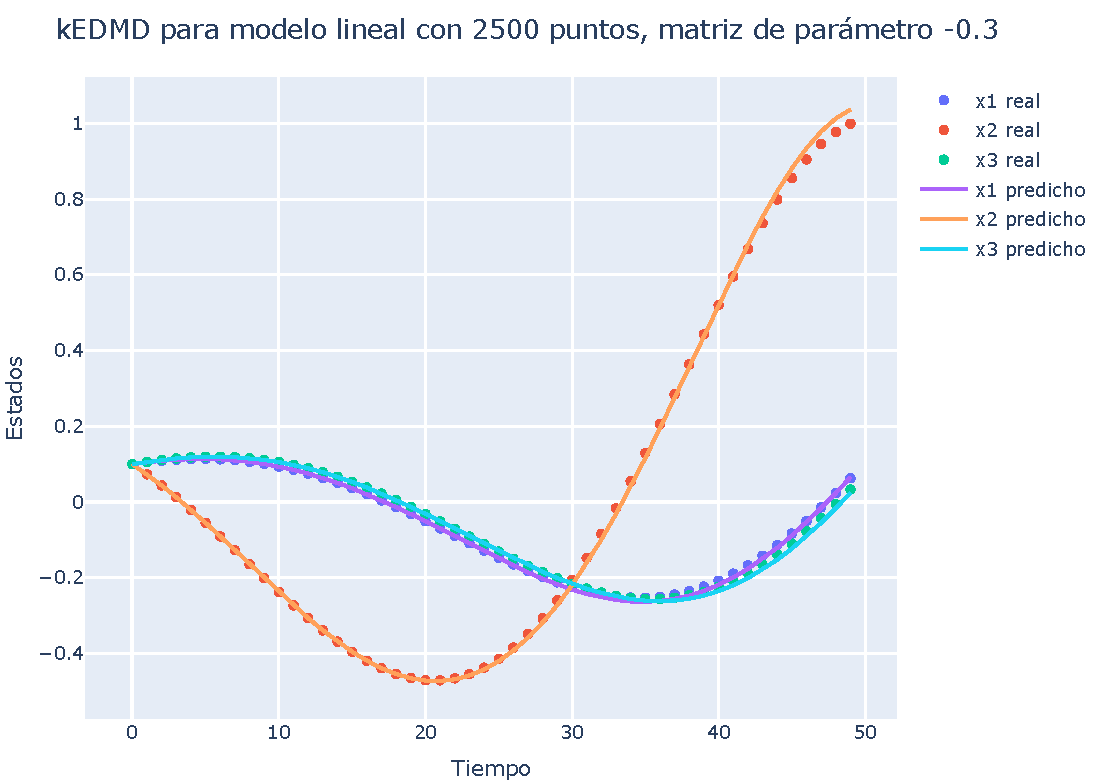
\includegraphics[width=\textwidth]{img/content/chapter3/Linear1.pdf}
        \caption{$\alpha=-0.3$}
        \label{fig:image1}
    \end{subfigure}
    \hfill
    \begin{subfigure}[b]{0.32\textwidth}
        \centering
        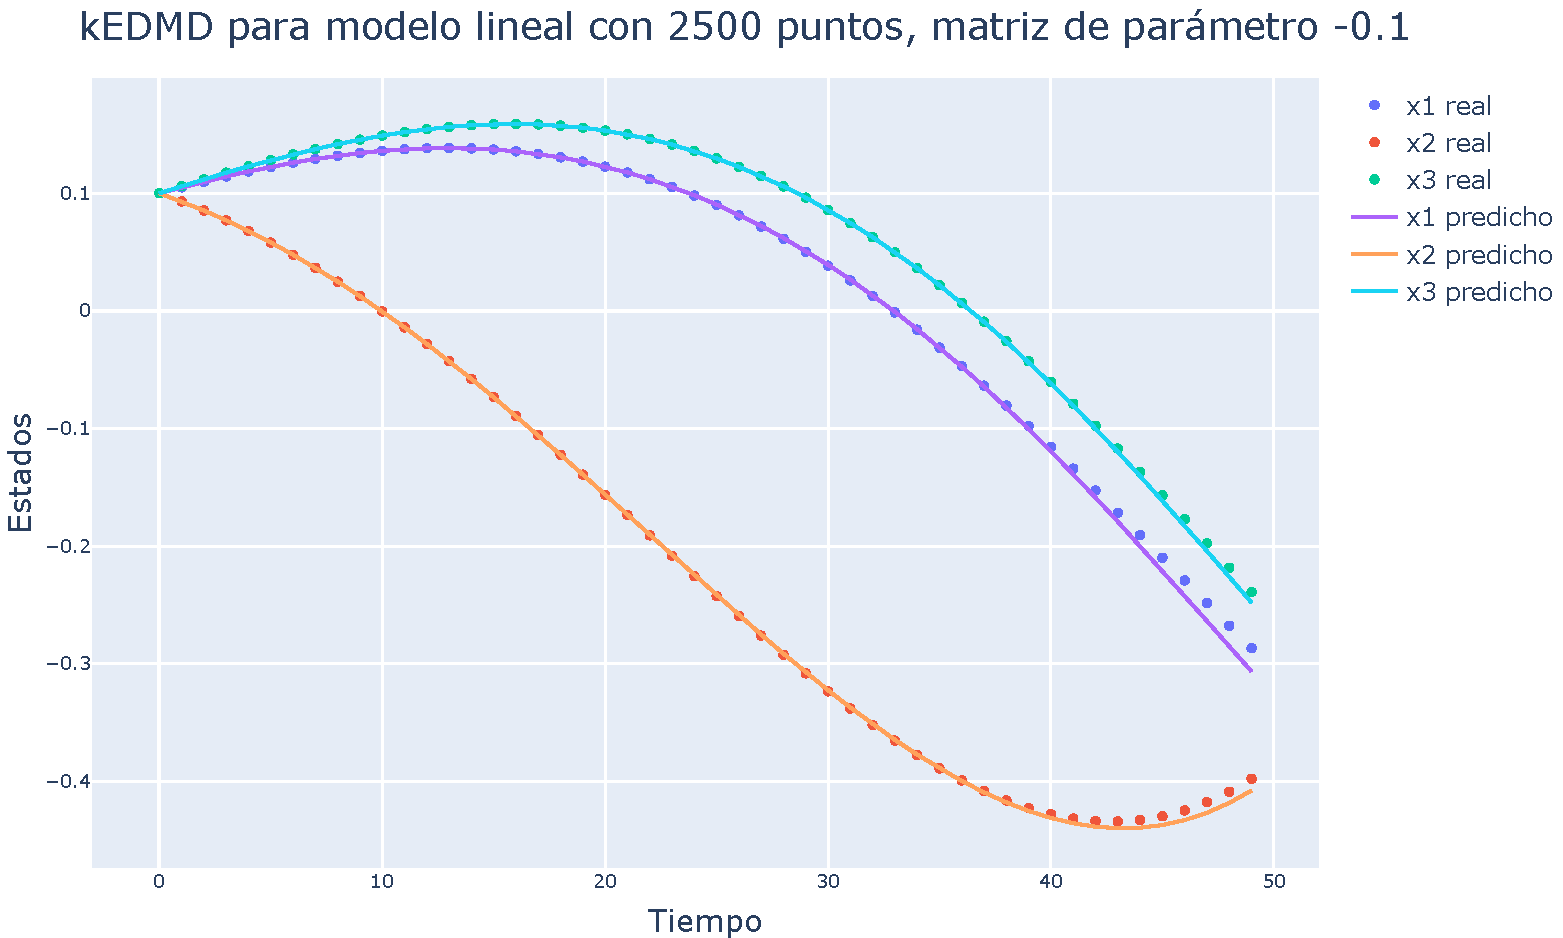
\includegraphics[width=\textwidth]{img/content/chapter3/Linear2.pdf}
        \caption{$\alpha=-0.1$}
        \label{fig:image2}
    \end{subfigure}
    \hfill
    \begin{subfigure}[b]{0.32\textwidth}
        \centering
        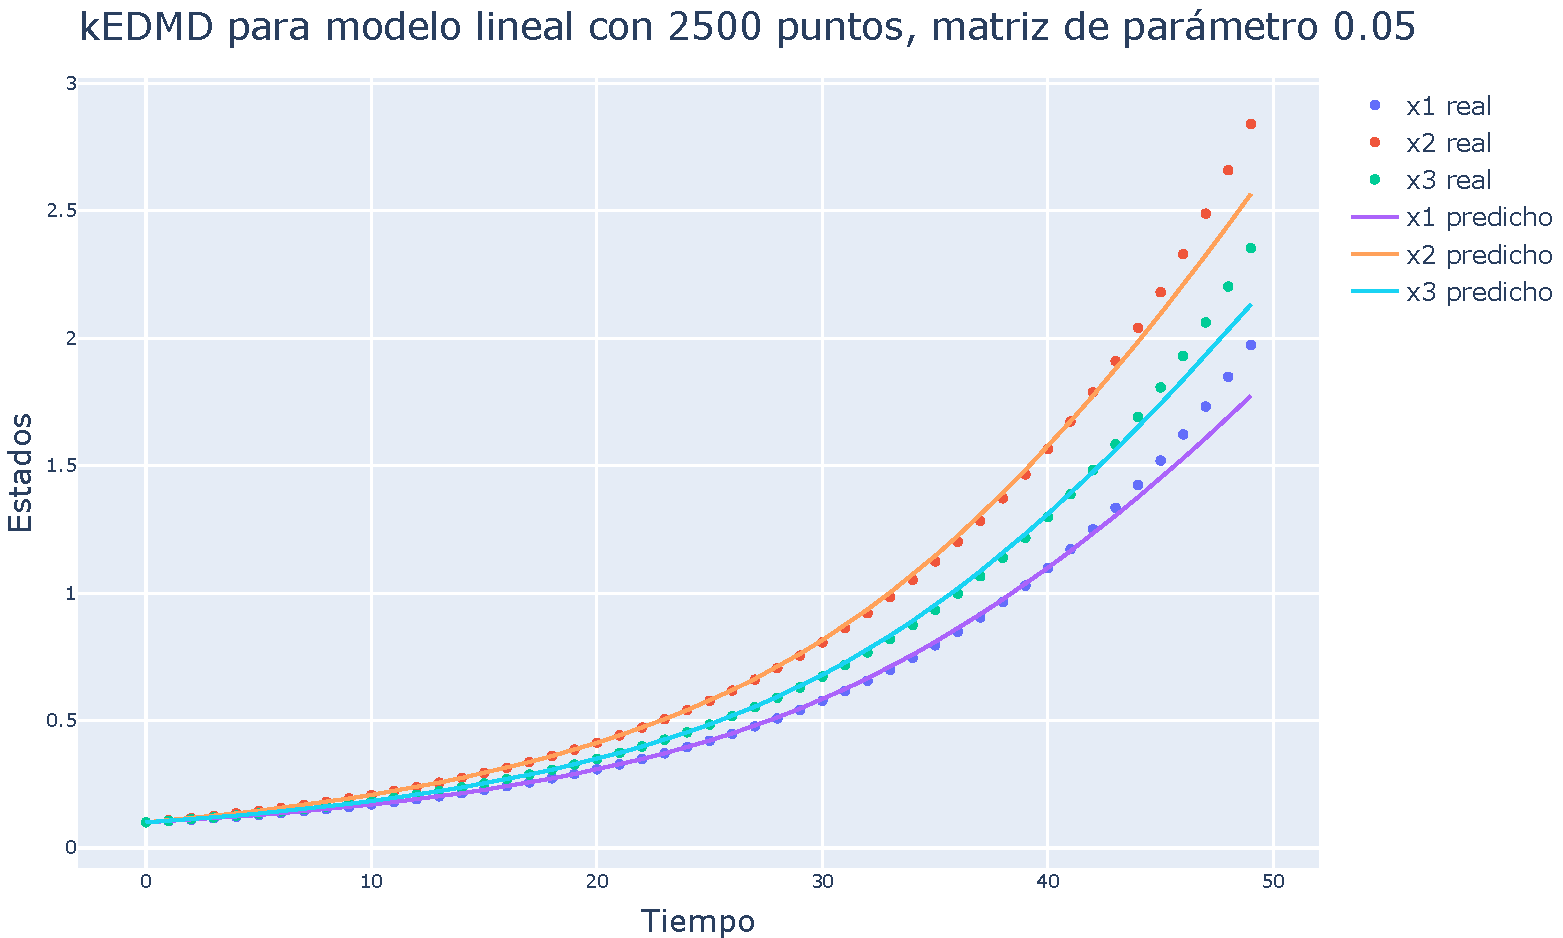
\includegraphics[width=\textwidth]{img/content/chapter3/Linear3.pdf}
        \caption{$\alpha=0.05$}
    \end{subfigure}
    \caption{Ilustración de los tres casos de $\alpha$ elegidos para la comparación entre el sistema lineal original y el sistema linealizado por Koopman a 2500 puntos \textit{sampleados} de una variable aleatoria normal. En forma de puntos se dejan los valores reales que toma el sistema y en línea continua los valores entregados por el sistema linealizado, que se consideran como predicción.}
    \label{fig:Comp_traj_lin}
\end{figure}
Aunque la cota en \eqref{eq:kEDMD_bound} no hace referencia directa a la diferencia en norma de las trayectorias, es de interés analizar el orden en que decae el error en función de $N$, para ello se calcula la diferencia en norma de las trayectorias generadas para $N \in \{ 100k : k \in \{1, \dots, 30\} \}$. \\
En la figura \ref{fig:Comp_traj_lin} se observa que las trayectorias obtenidas con el sistema linealizado vía Koopman son muy cercanas a las obtenidas con el sistema lineal original, solo difiriendo en zonas donde el sistema original toma valores muy altos, lo que se puede asociar a la poca probabilidad de \textit{sampleo} que le da la distribución normal elegida a puntos muy alejados del origen. \\
Mientras que en la figura \ref{fig:ErrorLin} se observa que en realidad el orden de decaimiento del error en función de $N$ es mayor que $N^{-1/2}$, mejorando la cota mostrada en \eqref{eq:kEDMD_bound}.
\begin{figure}[h]
    \centering
    \begin{subfigure}[b]{0.32\textwidth}
        \centering
        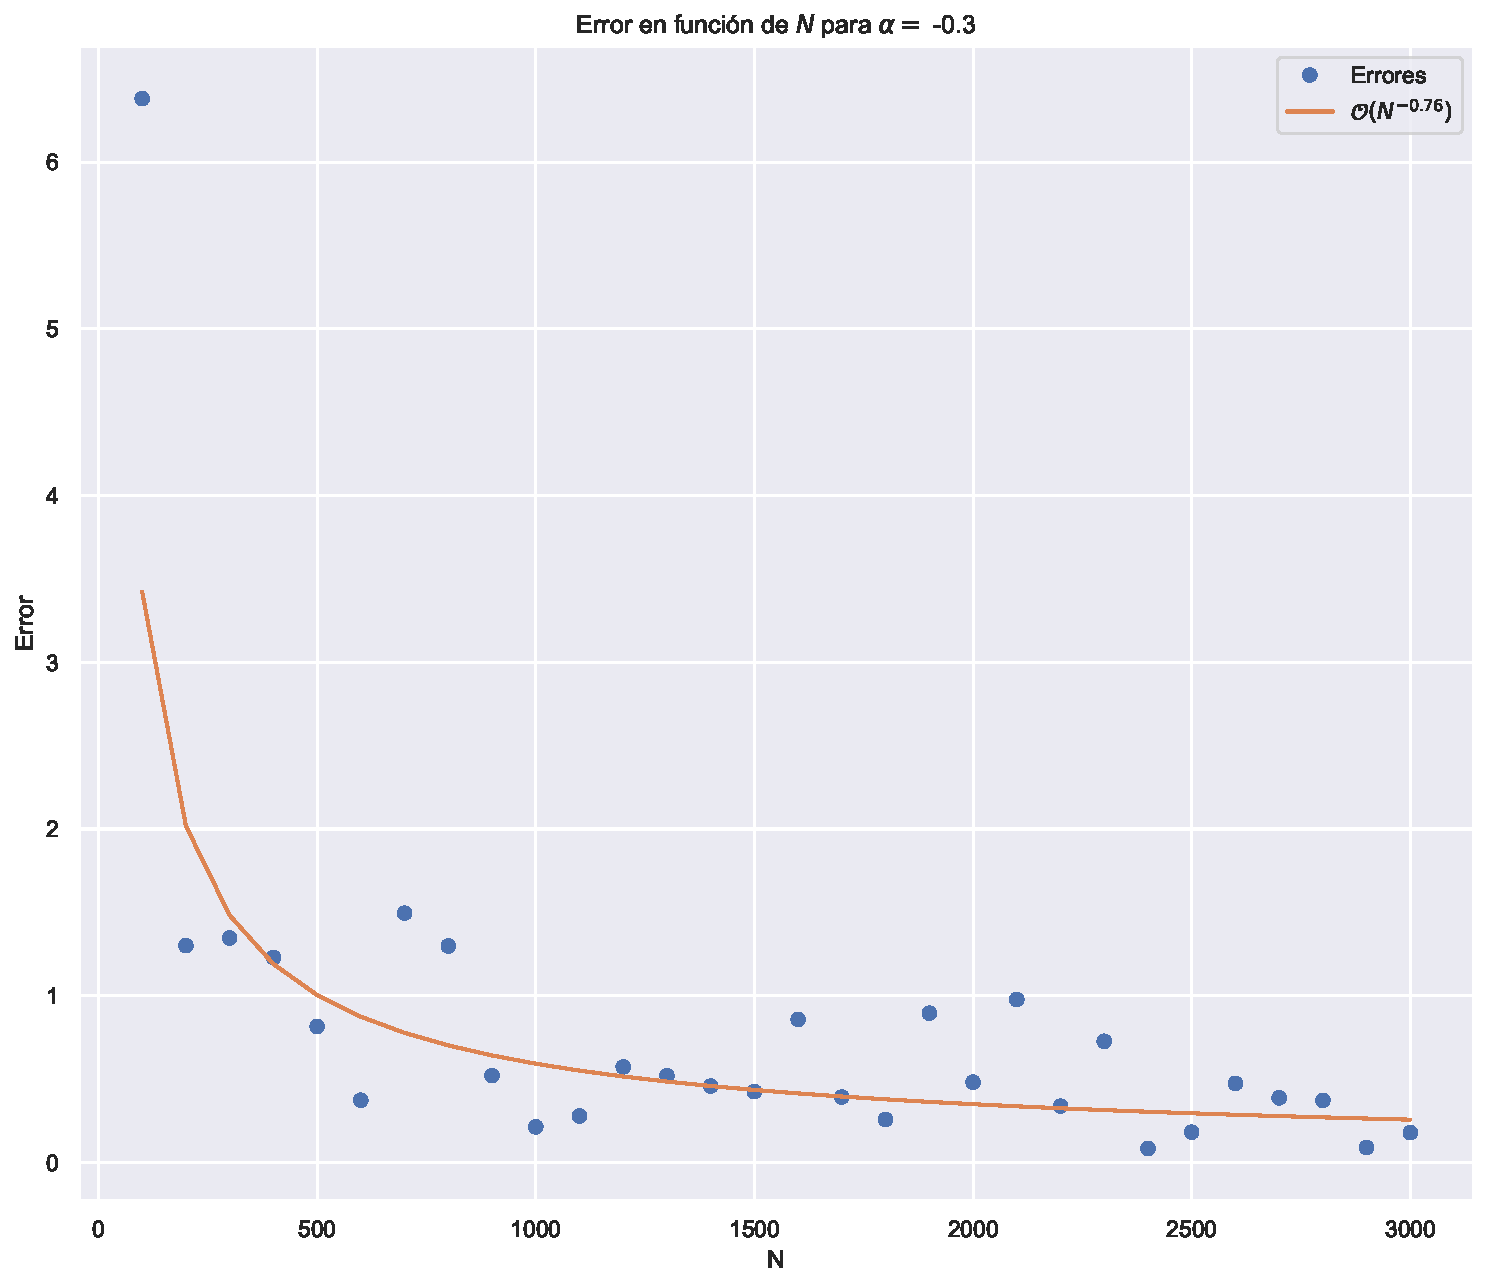
\includegraphics[width=\textwidth]{img/content/chapter3/Linear1Errors.pdf}
        \caption{$\alpha=-0.3$}
        \label{fig:image1}
    \end{subfigure}
    \hfill
    \begin{subfigure}[b]{0.32\textwidth}
        \centering
        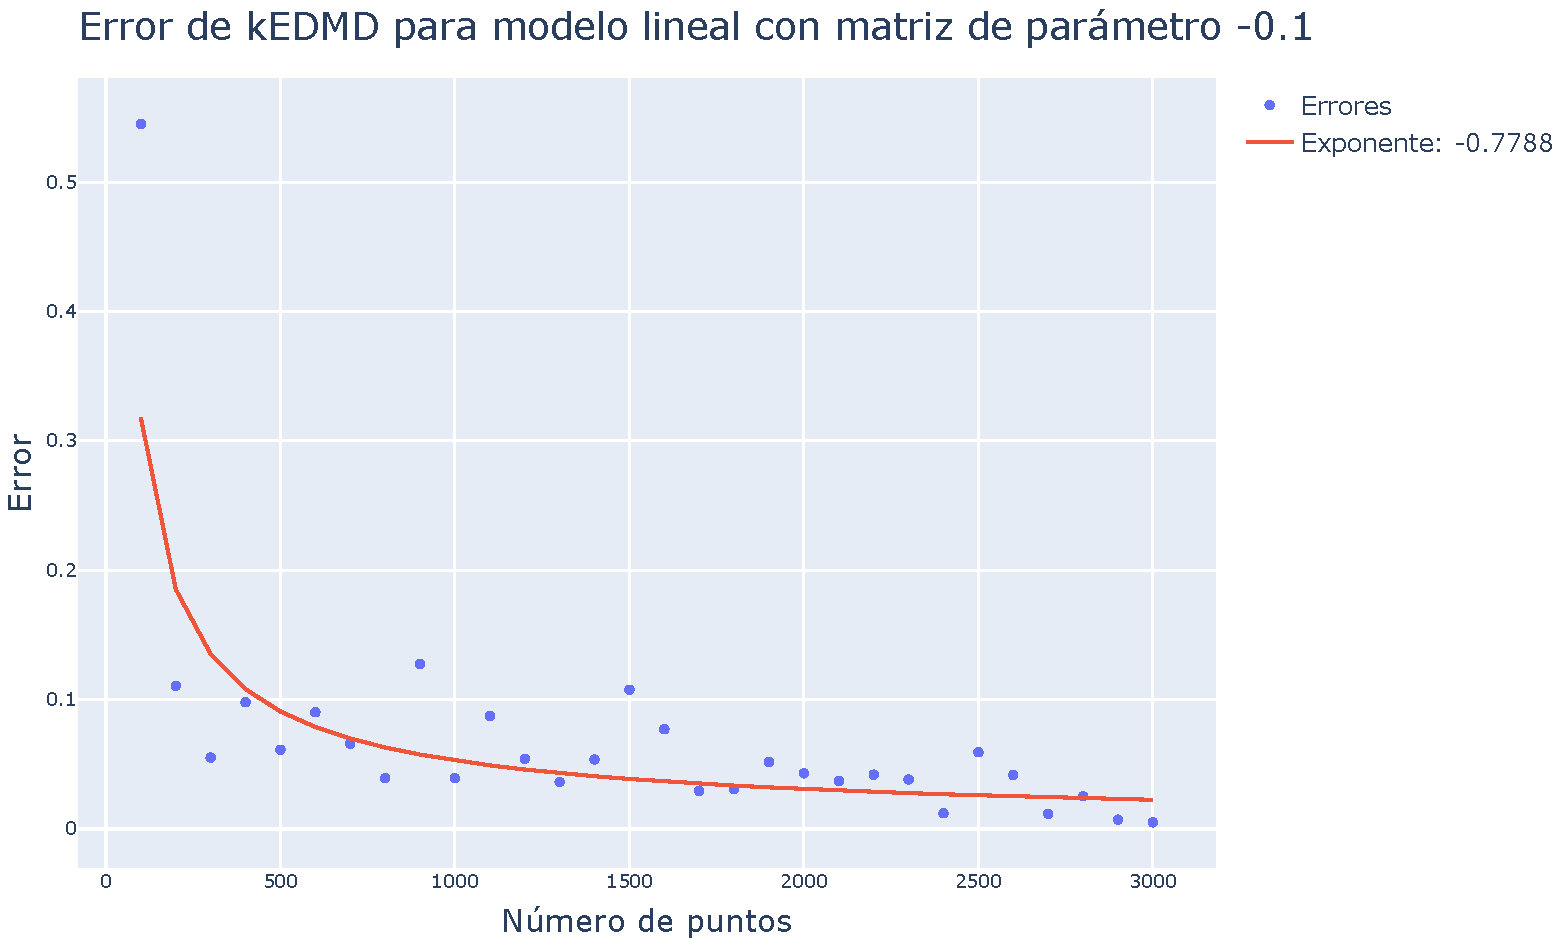
\includegraphics[width=\textwidth]{img/content/chapter3/Linear2Errors.pdf}
        \caption{$\alpha=-0.1$}
        \label{fig:image2}
    \end{subfigure}
    \hfill
    \begin{subfigure}[b]{0.32\textwidth}
        \centering
        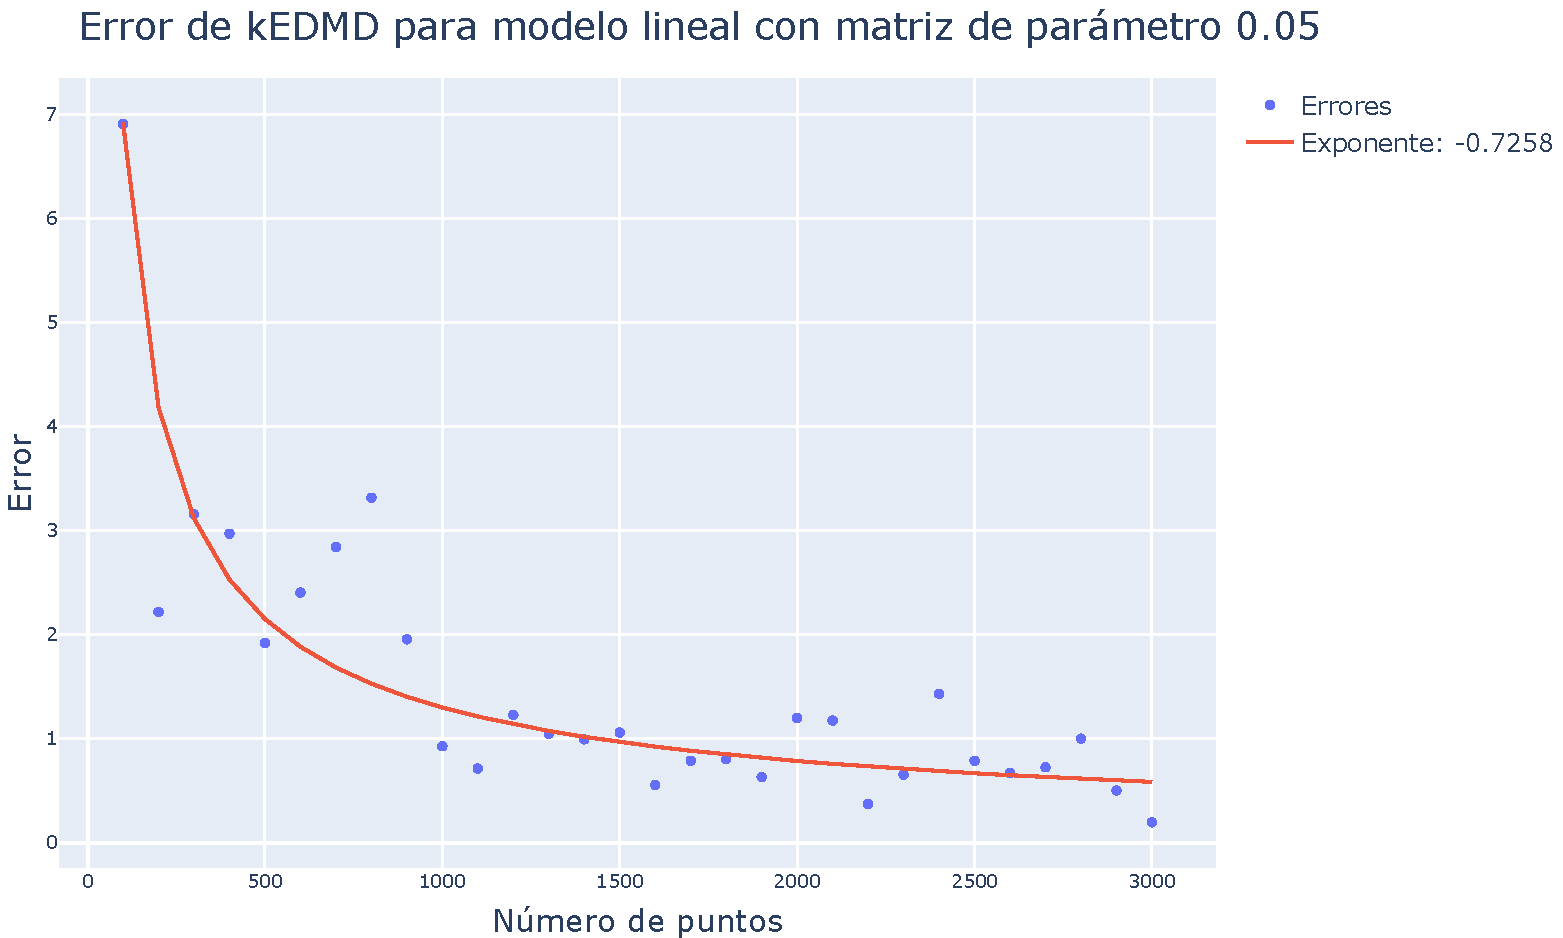
\includegraphics[width=\textwidth]{img/content/chapter3/Linear3Errors.pdf}
        \caption{$\alpha=0.05$}
        \label{fig:image3}
    \end{subfigure}
    \caption{Ilustración de los tres casos de $\alpha$ elegidos para la evolución en función de $N$ de la diferencia en norma entre el sistema lineal original y el sistema linealizado por Koopman a $N$ puntos \textit{sampleados} de una variable aleatoria normal. En forma de puntos se deja la evolución observada del error y en línea continua la mejor curva de la forma $C \cdot N^{a}$, donde $a$ es el exponente que se deja en la leyenda.}
    \label{fig:ErrorLin}
\end{figure}
\subsection{kEDMD para modelos utilizados en epidemiología}
Para esta sección se ilustrarán los resultados de kEDMD para modelos epidemiológicos que no consideran nacimientos ni muertes, es decir, su población total se mantiene constante en el tiempo. Estos modelos reciben el nombre de compartimentales, ya que cada parte de la población se encuentra en un único compartimento y toda la población está en alguno de ellos. Para estos casos se supondrá que la población está normalizada, esto es, que cada compartimento está en $[0, 1]$.\\
Esto último permite decir que el espacio de estados de este modelo es, sin considerar los eventuales factores estocásticos, un $(n-1)$-simplex, siendo $n$ la cantidad de compartimentos considerados, que se define como el conjunto
\begin{equation*}
    \Delta_{n-1} = \left \{ x \in \R^n : \sum_{i=1}^n x_i = 1, \, x_i \geq 0, \, \forall i \in \{1, \dots, n\} \right \}.
\end{equation*}
De este conjunto se puede \textit{samplear} de manera eficiente desde una distribución Dirichlet \cite{Frigyik2010IntroductionProcesses}, y se encuentra implementado en las principales librerías con funcionalidades estadísticas como SciPy \cite{Virtanen2020SciPyPython}, que será la utilizada en este trabajo.\\
La densidad de una variable aleatoria Dirichlet con parámetros $\alpha_1, \alpha_2, \ldots, \alpha_K$ se define como:
\[
f(x_1, x_2, \ldots, x_K; \alpha_1, \alpha_2, \ldots, \alpha_K) = \frac{1}{B(\alpha)} \prod_{i=1}^{K} x_i^{\alpha_i - 1}
\]
donde $x_i \geq 0$ para todo $i$, $\sum_{i=1}^{K} x_i = 1$, y
\[
B(\alpha) = \frac{\prod_{i=1}^{K} \Gamma(\alpha_i)}{\Gamma\left(\sum_{i=1}^{K} \alpha_i\right)}
\]
es la función beta multivariable, y $\Gamma(\cdot)$ es la función gamma. En la figura \ref{fig:Dirichlet_samples} se puede apreciar la diferencia de \textit{samplear} para diferentes valores de $\alpha$. Un valor de $\alpha$ con entradas iguales genera la misma dispersión en todas las direcciones, siendo $(1, 1, 1)$ la variable aleatoria uniforme en $\Delta_{n-1}$, mientras que valores altos de $\alpha$ generan una alta concentración de muestras en el centro del conjunto. Por otro lado valores desiguales generar mayor cantidad de muestras en alguna de las caras del conjunto.
\begin{figure}[htbp]
    \centering
    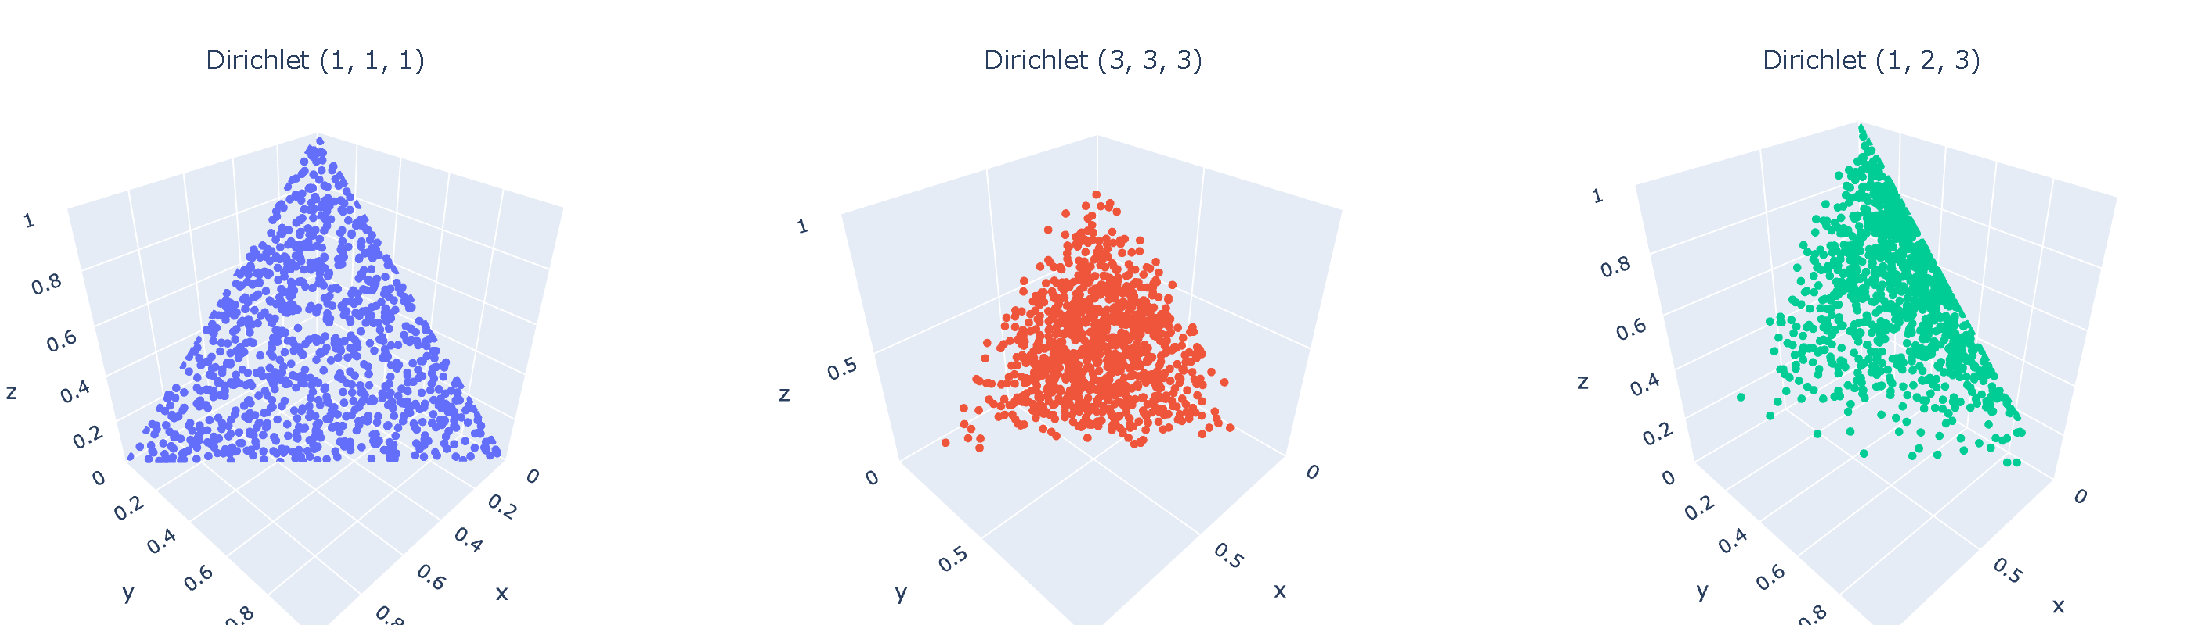
\includegraphics[width=0.95\linewidth]{img/content/chapter3/Dirichlet.pdf}
    \caption{1000 muestras de una variable aleatoria Dirichlet para diferentes valores de $\alpha$, observando dos casos de $\alpha$ con valores homogéneos y uno con valores heterogéneos, lo que provoca un desbalance de muestras.}
    \label{fig:Dirichlet_samples}
\end{figure}
El primer ejemplo clásico es el modelo SIR, en donde se supone que se tiene una dinámica de contagios tal que los susceptibles y los infectados interactúan y a cierta tasa se generan más contagios; luego, a cierta tasa, estos infectados se recuperan, ganan inmunidad y por tanto son removidos de la dinámica de contagio, por lo que no vuelven a ser susceptibles.\\
En tiempo discreto, la dinámica de este modelo viene dada por las ecuaciones
\begin{equation}
    \begin{aligned}
    S_{k+1} &= S_k -\beta S_k I_k, \\
    I_{k+1} &= I_k + \beta S_k I_k - \gamma I_k, \\
    S_{k+1} &= R_k + \gamma I_k,
    \end{aligned}
    \label{eq:SIR}
\end{equation}
donde:
\begin{itemize}
    \item \(S_k\) es el número de individuos susceptibles en el tiempo k,
    \item \(I_k\) es el número de individuos infecciosos en el tiempo \(k\),
    \item \(R_k\) es el número de individuos recuperados en el tiempo \(k\),
    \item \(\beta\) es la tasa de transmisión de la enfermedad,
    \item \(\gamma\) es la tasa de recuperación.
\end{itemize}
Se visualiza lo obtenido por kEDMD, utilizando \textit{kernel} de Matérn de parámetro $\nu=1/2$ y ancho de banda $\gamma=10^{-3}$. Se utiliza una distribución Dirichlet de parámetro $(1,1,1)$ como variable aleatoria asociada al espacio de estados y ruido aditivo centrado y Gaussiano de matriz de covarianza $10^{-7} I_{3 \times 3}$, de estas distribuciones se \textit{samplearán} $N=1000$ puntos. Se toma como condición inicial $\mathbf{x}_0 = (0.9, 0.1, 0.0)$ y los resultados obtenidos se pueden ver en la imagen \ref{fig:Comp_traj_SIR}. \\
\begin{figure}[htbp]
    \centering
    \begin{subfigure}[b]{0.45\textwidth}
        \centering
        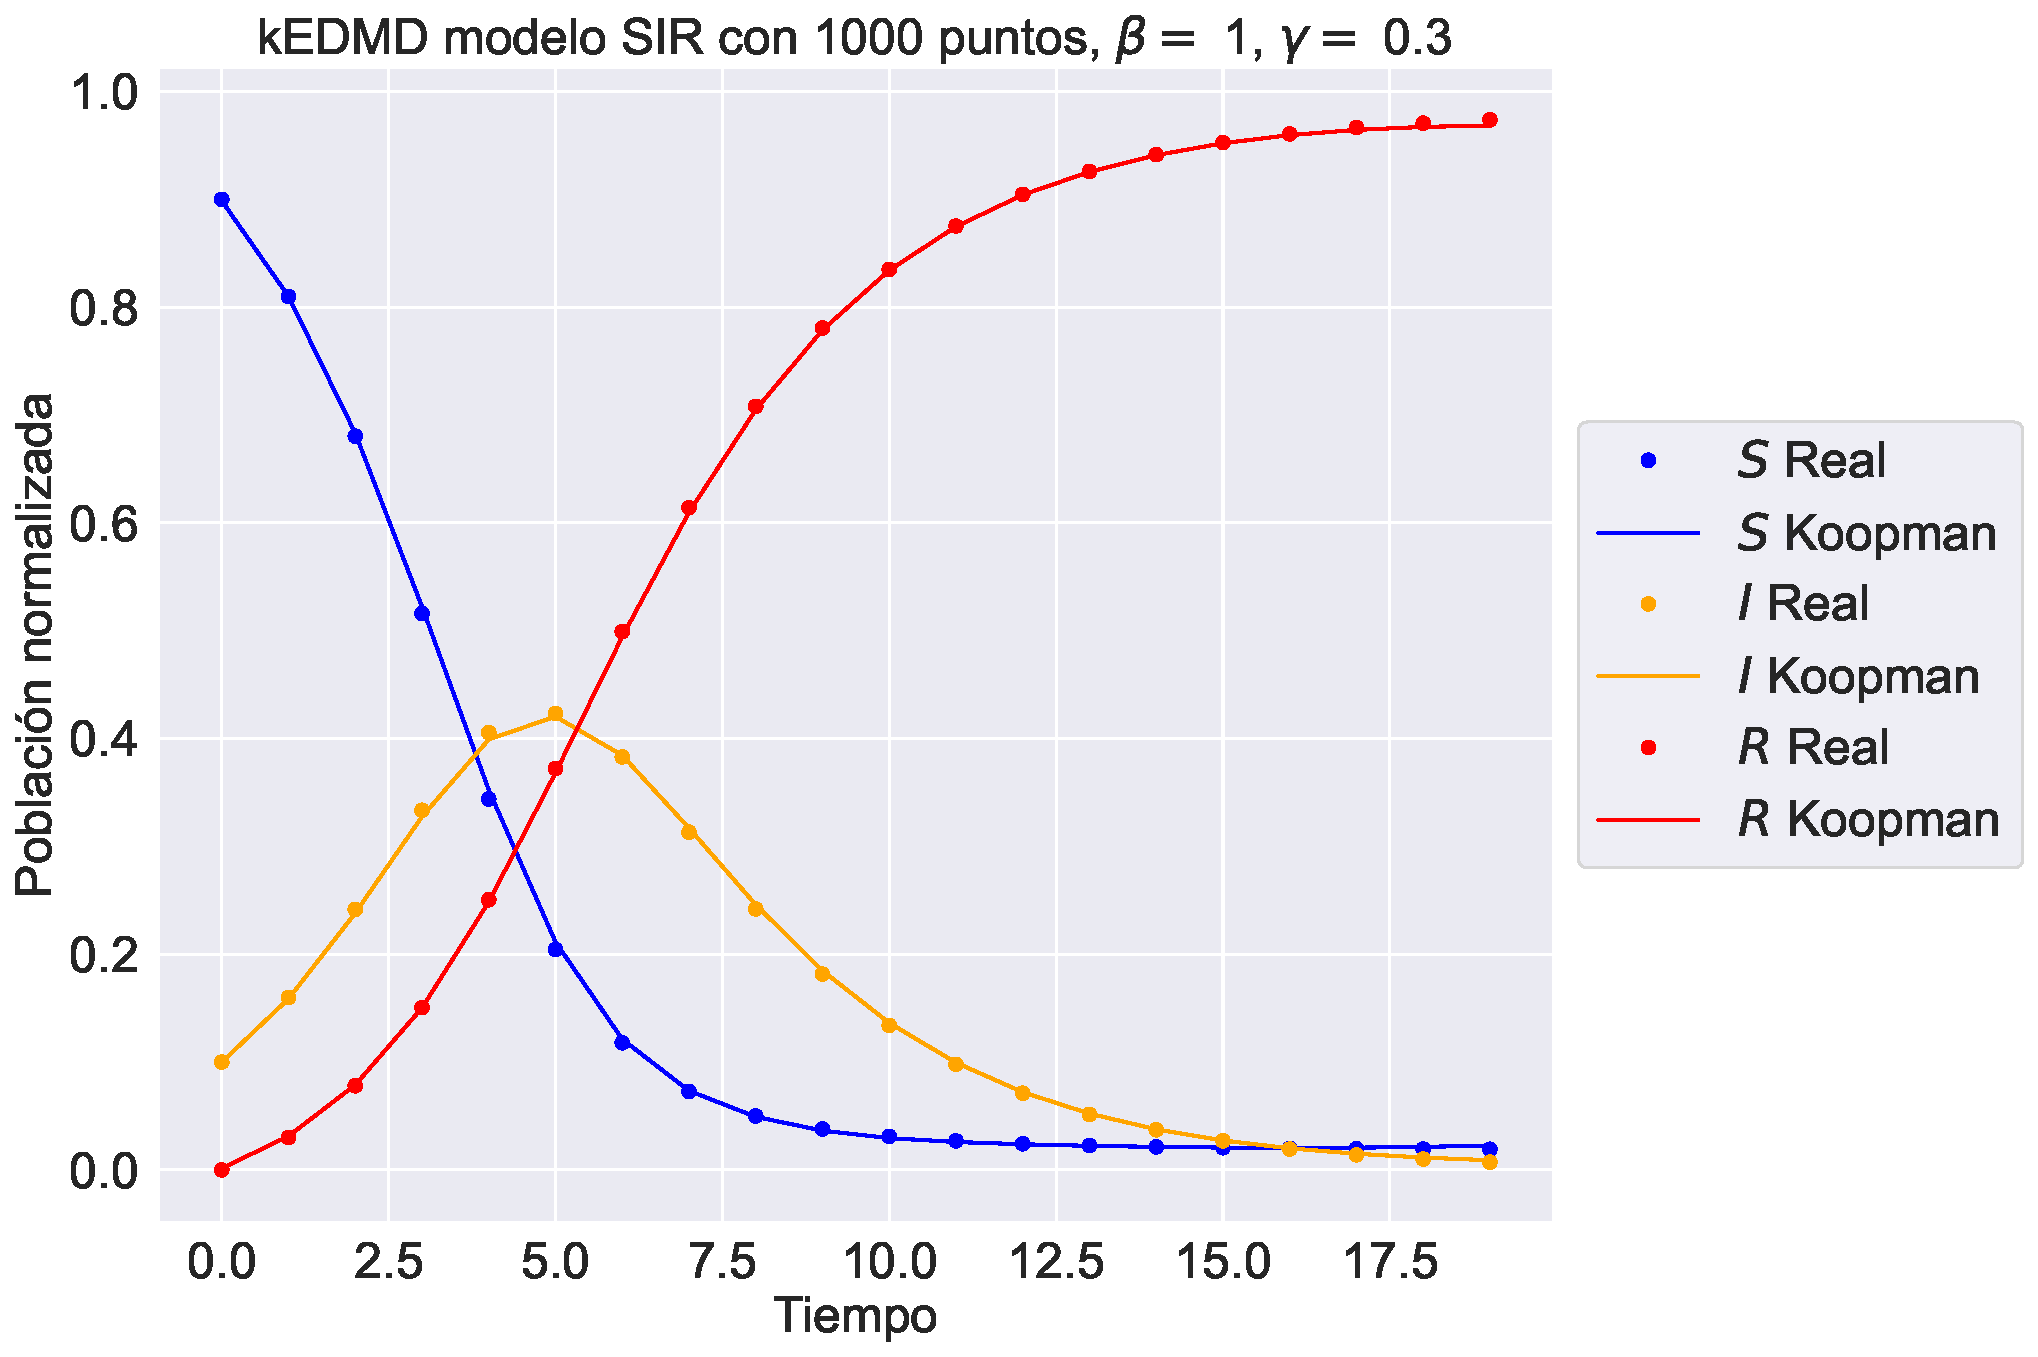
\includegraphics[width=\textwidth]{img/content/chapter3/SIR1.pdf}
        \caption{$\alpha=-0.3$}
        \label{fig:image1}
    \end{subfigure}
    \hfill
    \begin{subfigure}[b]{0.45\textwidth}
        \centering
        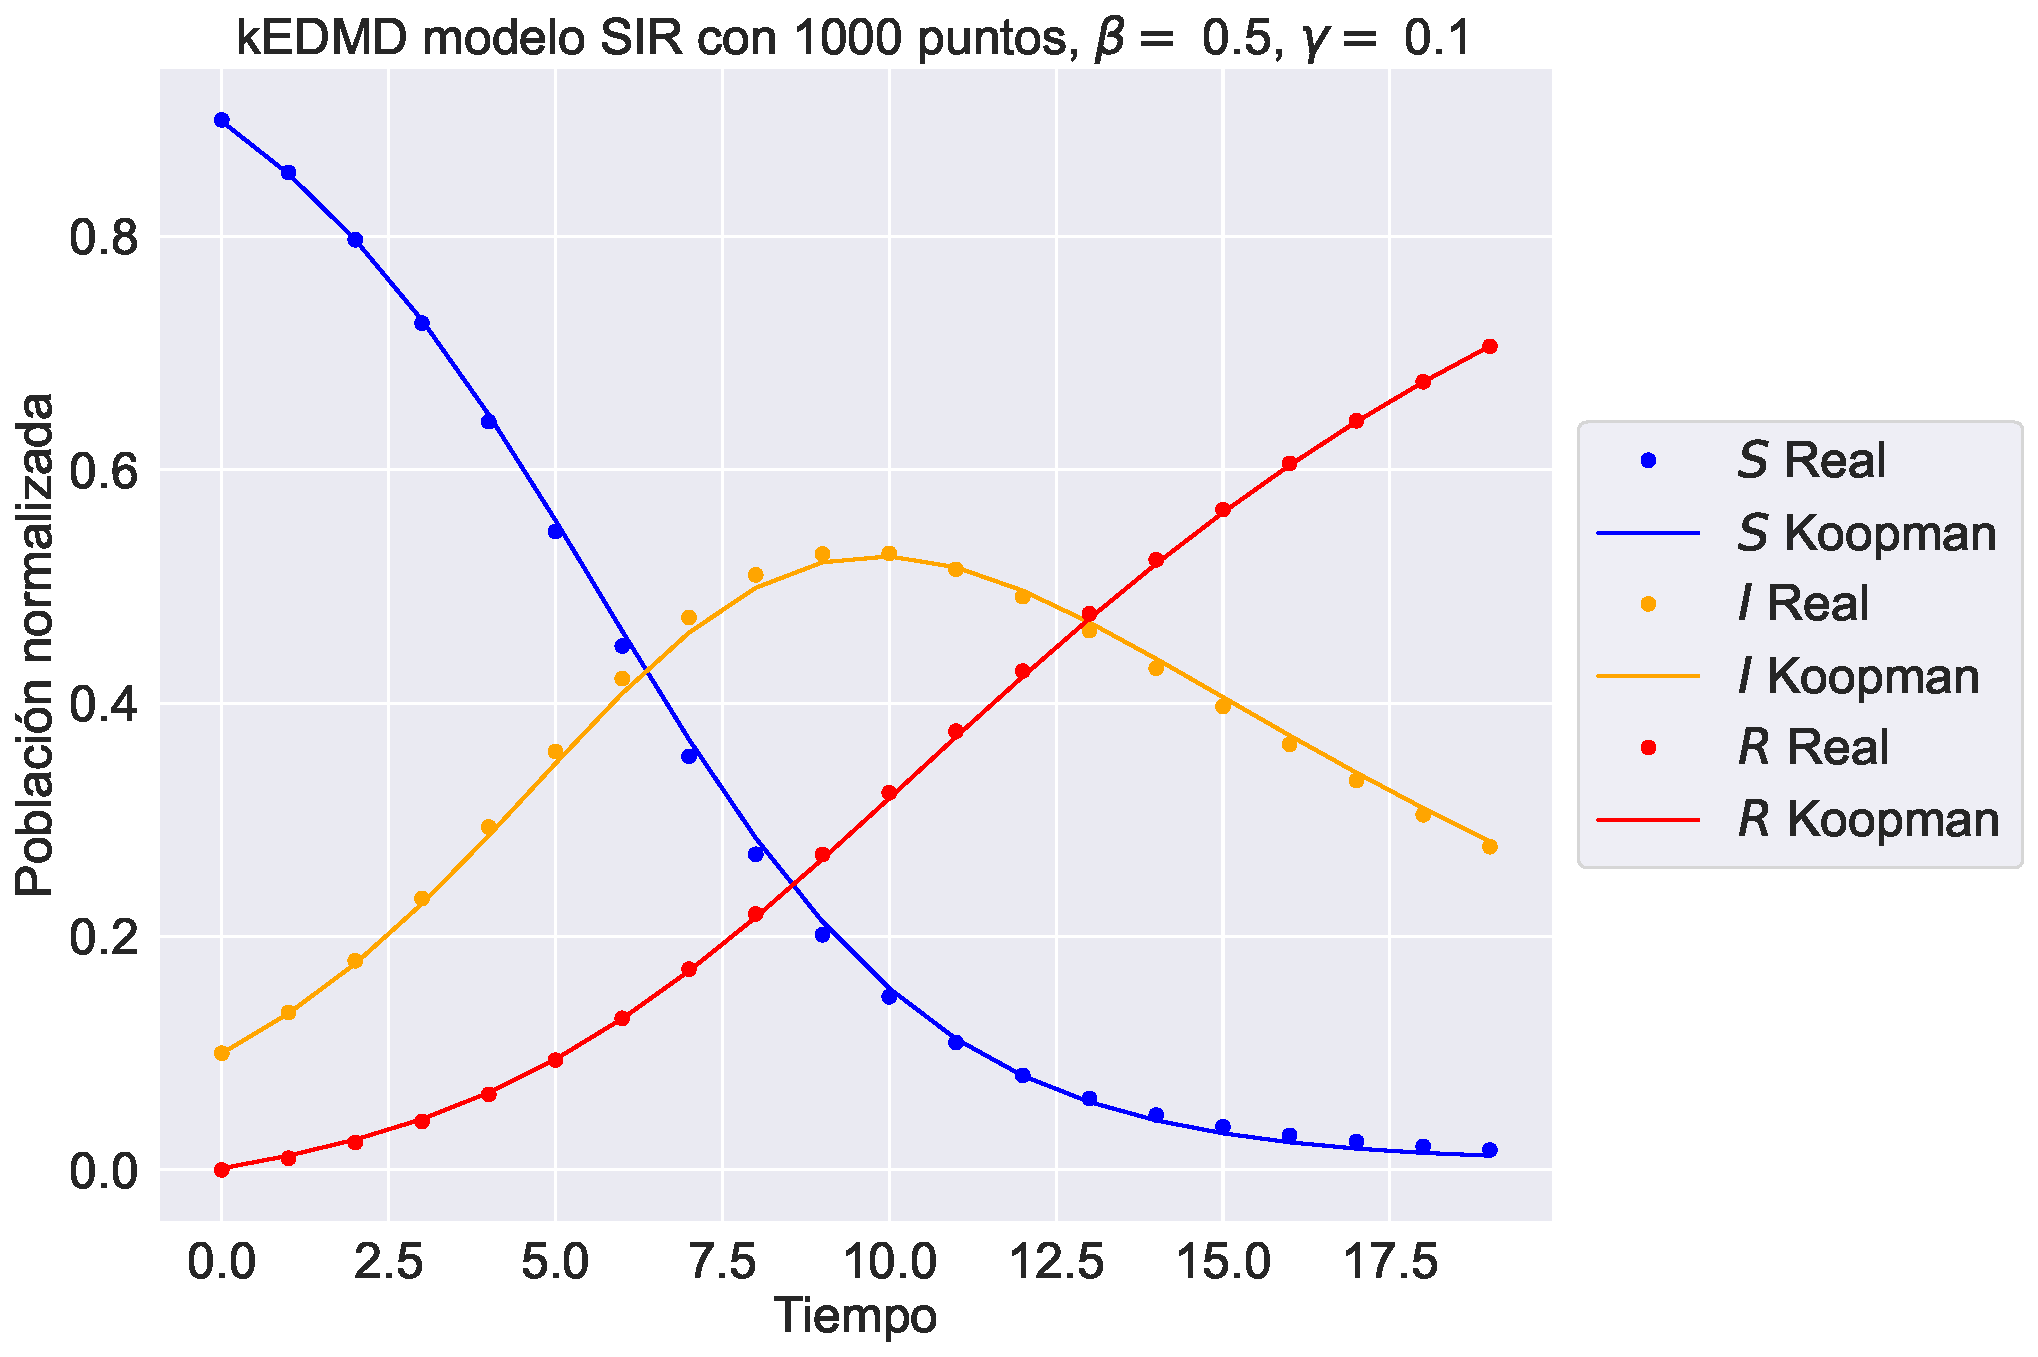
\includegraphics[width=\textwidth]{img/content/chapter3/SIR2.pdf}
        \caption{$\alpha=-0.1$}
        \label{fig:image2}
    \end{subfigure}
    \hfill
    \begin{subfigure}[b]{0.45\textwidth}
        \centering
        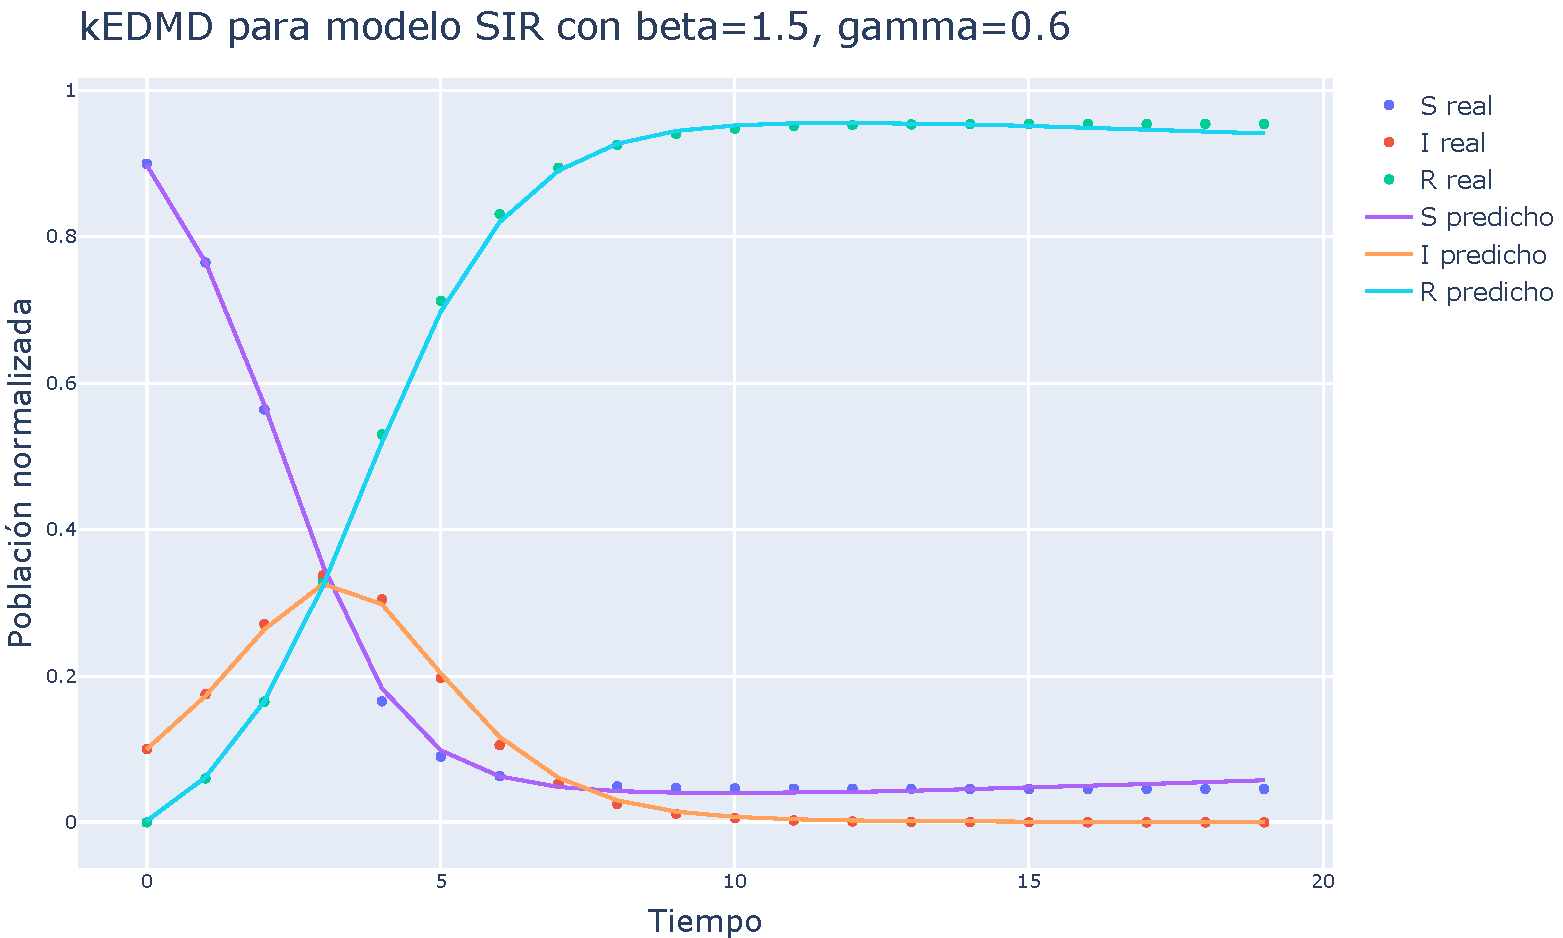
\includegraphics[width=\textwidth]{img/content/chapter3/SIR3.pdf}
        \caption{$\alpha=0.05$}
    \end{subfigure}
    \caption{Ilustración de los tres casos de $\beta$ y $\gamma$ elegidos para la comparación entre el sistema no lineal original y el sistema linealizado por Koopman a 1000 puntos \textit{sampleados} de una variable aleatoria Dirichlet. En forma de puntos se dejan los valores reales que toma el sistema y en línea continua los valores entregados por el sistema linealizado, que se consideran como predicción.}
    \label{fig:Comp_traj_SIR}
\end{figure}
Similar a lo hecho en el caso lineal, en la figura \ref{fig:ErrorSIR} se compara la diferencia en norma entre la trayectoria original y la trayectoria linealizada, con la mejor curva de la forma $C \cdot N^{a}$, para observar si los errores andan en el orden de decaimiento en \eqref{eq:kEDMD_bound}.
\begin{figure}[h]
    \centering
    \begin{subfigure}[b]{0.32\textwidth}
        \centering
        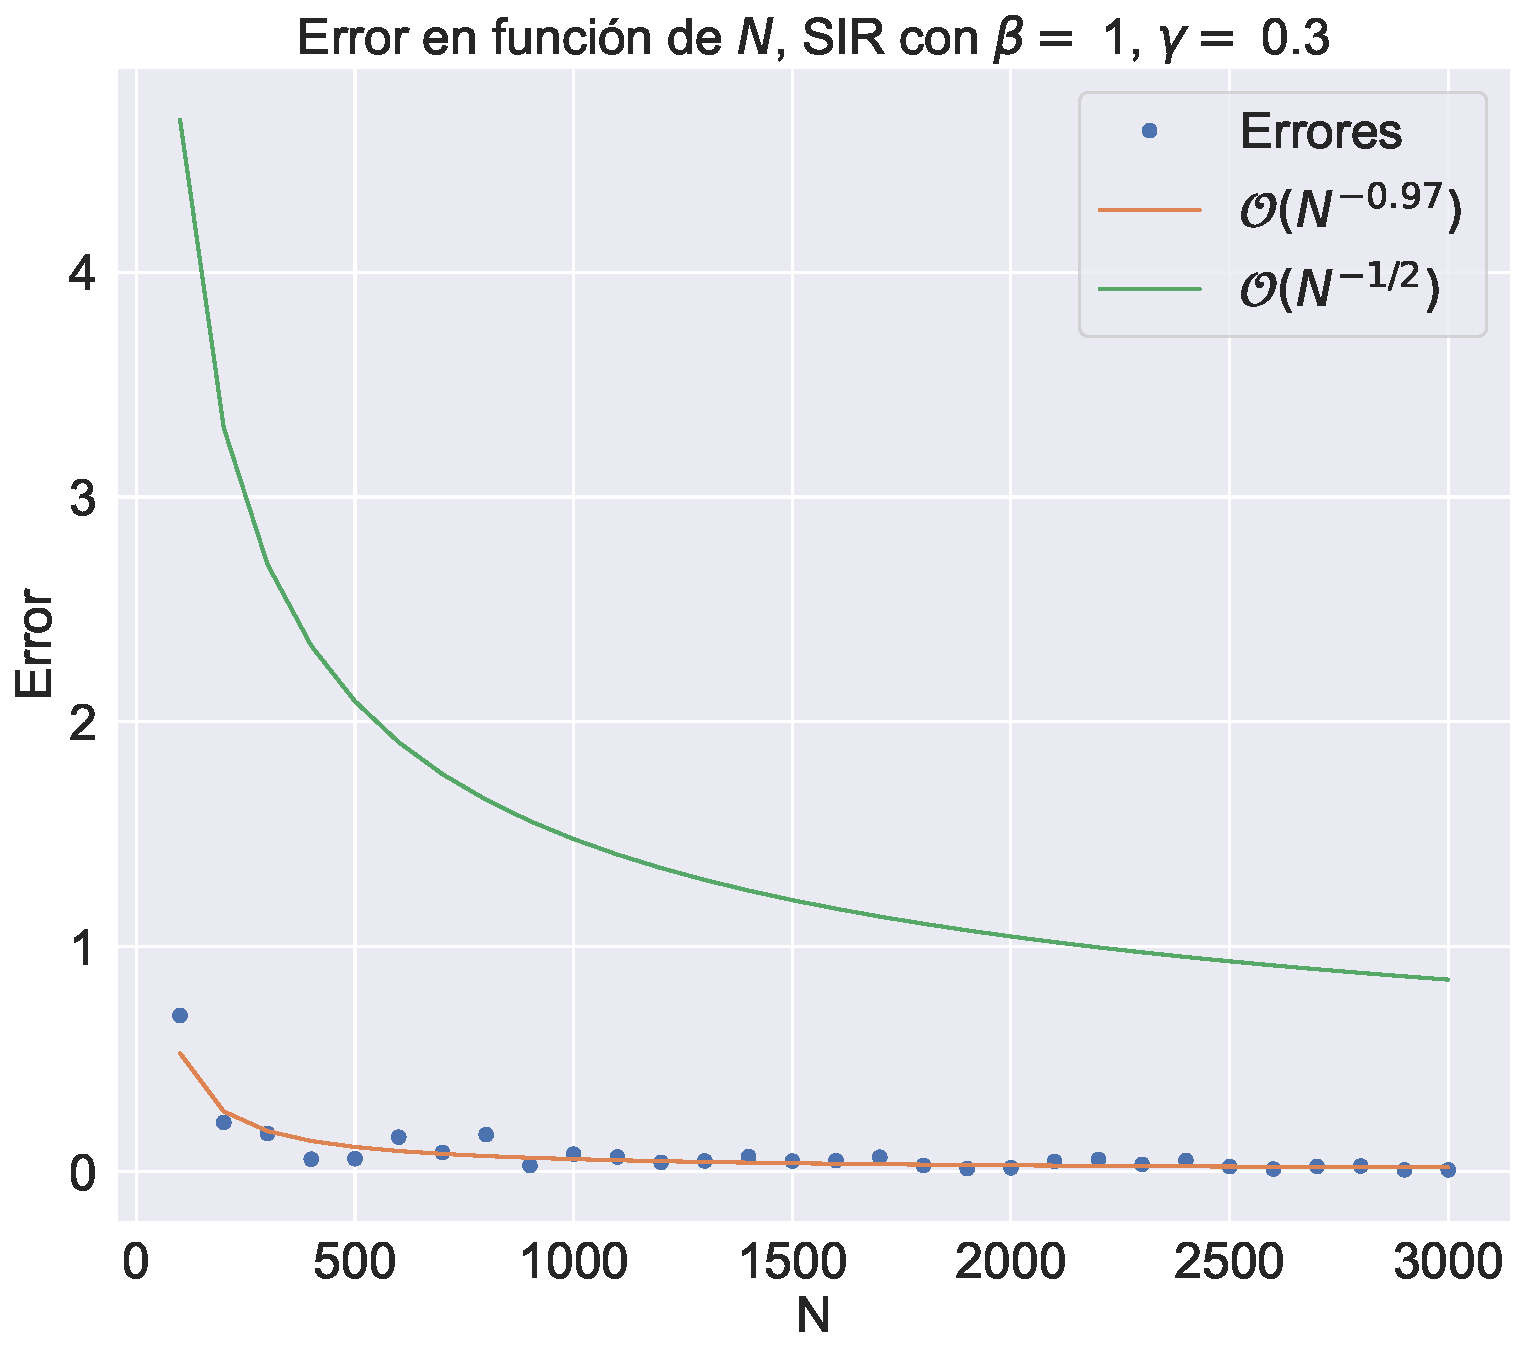
\includegraphics[width=\textwidth]{img/content/chapter3/SIR1Errors.pdf}
        \caption{$\beta=-0.3$, $\gamma=0.3$}
    \end{subfigure}
    \hfill
    \begin{subfigure}[b]{0.32\textwidth}
        \centering
        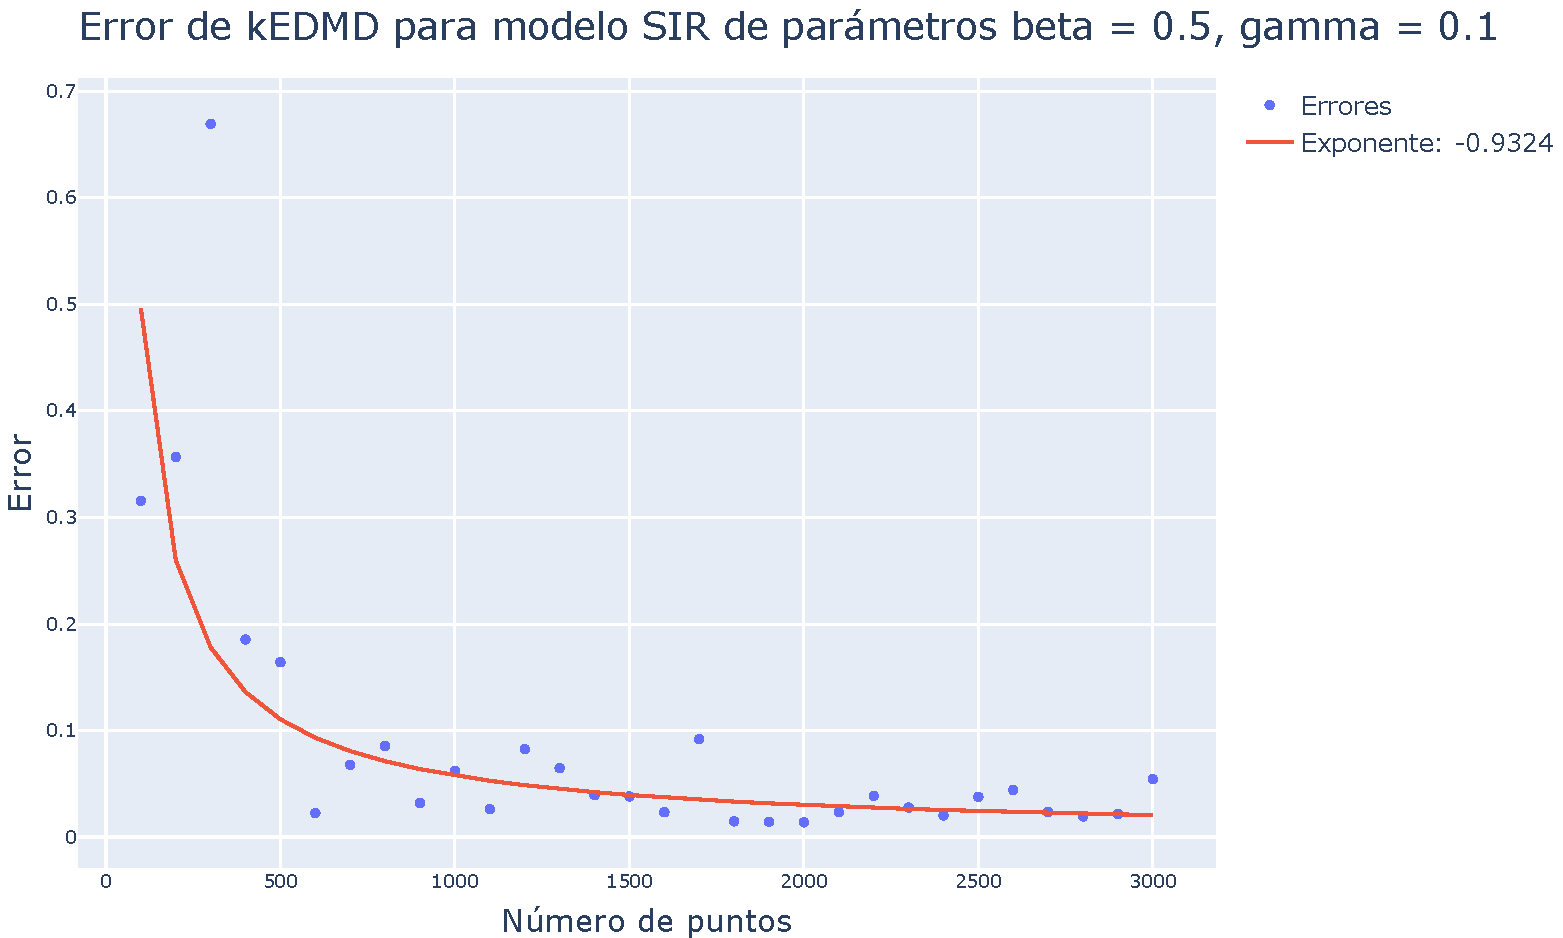
\includegraphics[width=\textwidth]{img/content/chapter3/SIR2Errors.pdf}
        \caption{$\beta=0.5$, $\gamma=0.1$}
    \end{subfigure}
    \hfill
    \begin{subfigure}[b]{0.32\textwidth}
        \centering
        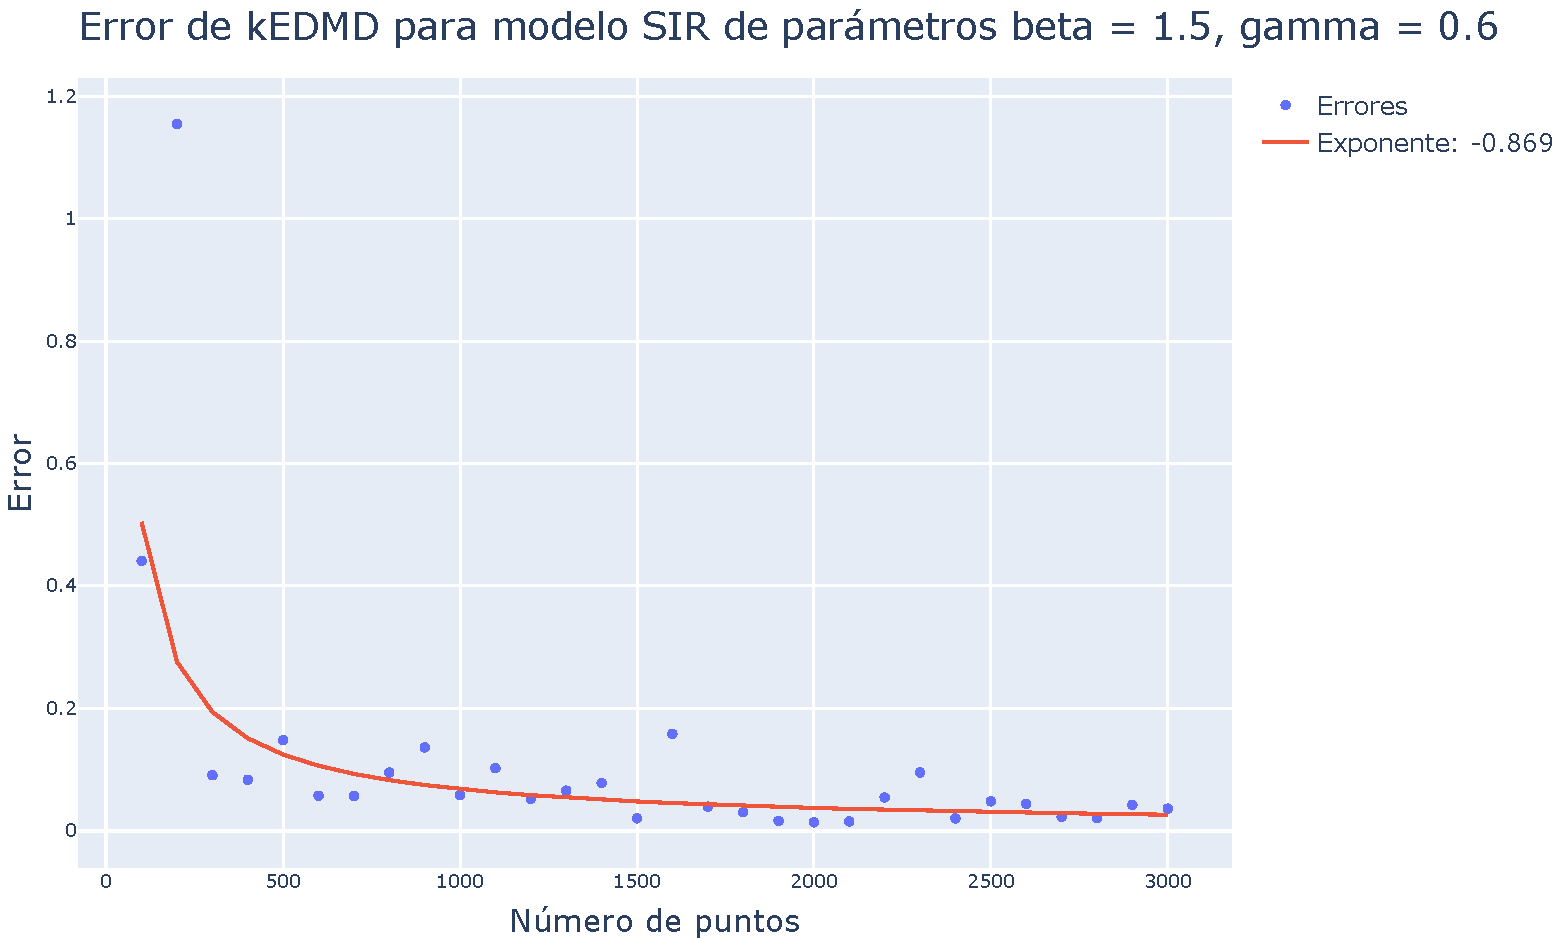
\includegraphics[width=\textwidth]{img/content/chapter3/SIR3Errors.pdf}
        \caption{$\beta=1.5$, $\gamma=0.6$}
    \end{subfigure}
    \caption{Ilustración de los tres casos del modelo SIR elegido para la evolución en función de $N$ de la diferencia en norma entre el sistema lineal original y el sistema linealizado por Koopman a $N$ puntos,  \textit{sampleados} de una variable aleatoria normal. En forma de puntos se deja la evolución observada del error y en línea continua la mejor curva de la forma $C \cdot N^{a}$, donde $a$ es el exponente que se deja en la leyenda.}
    \label{fig:ErrorSIR}
\end{figure}
Se observa nuevamente que la discrepancia entre las trayectorias en efecto anda del orden de la cota expuesta en este capítulo, incluso con decaimientos aún más rápidos.\\
Con ello, de manera sencilla puede incluirse un factor de pérdida de inmunidad, lo que viene dado por las ecuaciones
\begin{equation}
    \begin{aligned}
    S_{k+1} &= S_k -\beta S_k I_k + \alpha R_k, \\
    I_{k+1} &= I_k + \beta S_k I_k - \gamma I_k, \\
    S_{k+1} &= R_k + \gamma I_k - \alpha R_k,
    \end{aligned}
    \label{eq:SIR_rec}
\end{equation}
En donde el nuevo parámetro $\alpha$ es la tasa de pérdida de inmunidad después de haberse recuperado de la enfermedad y que no debe ser confundido con el parámetro de la variable aleatoria Dirichlet vista antes.
Se comparan las trayectorias generadas por el sistema original con las generadas por kEDMD, utilizando exactamente la misma configuración del sistema anterior, solo cambiando la dinámica.
\begin{figure}[h]
    \centering
    \begin{subfigure}[b]{0.45\textwidth}
        \centering
        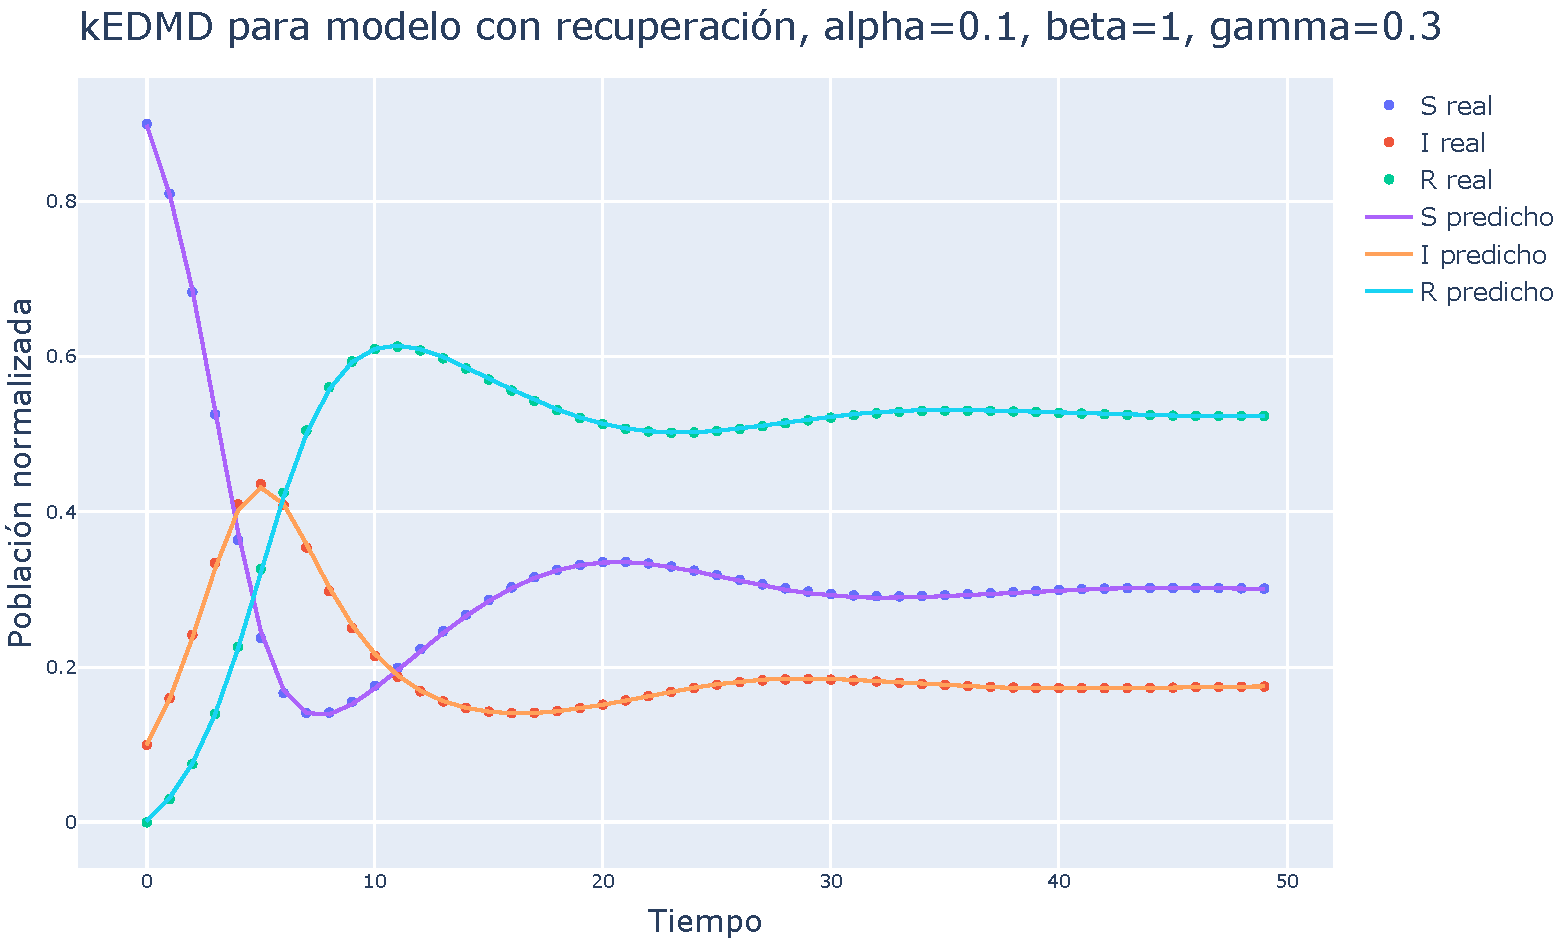
\includegraphics[width=\textwidth]{img/content/chapter3/SIR_rec1.pdf}
        \caption{$\alpha=-0.3$}
        \label{fig:image1}
    \end{subfigure}
    \hfill
    \begin{subfigure}[b]{0.45\textwidth}
        \centering
        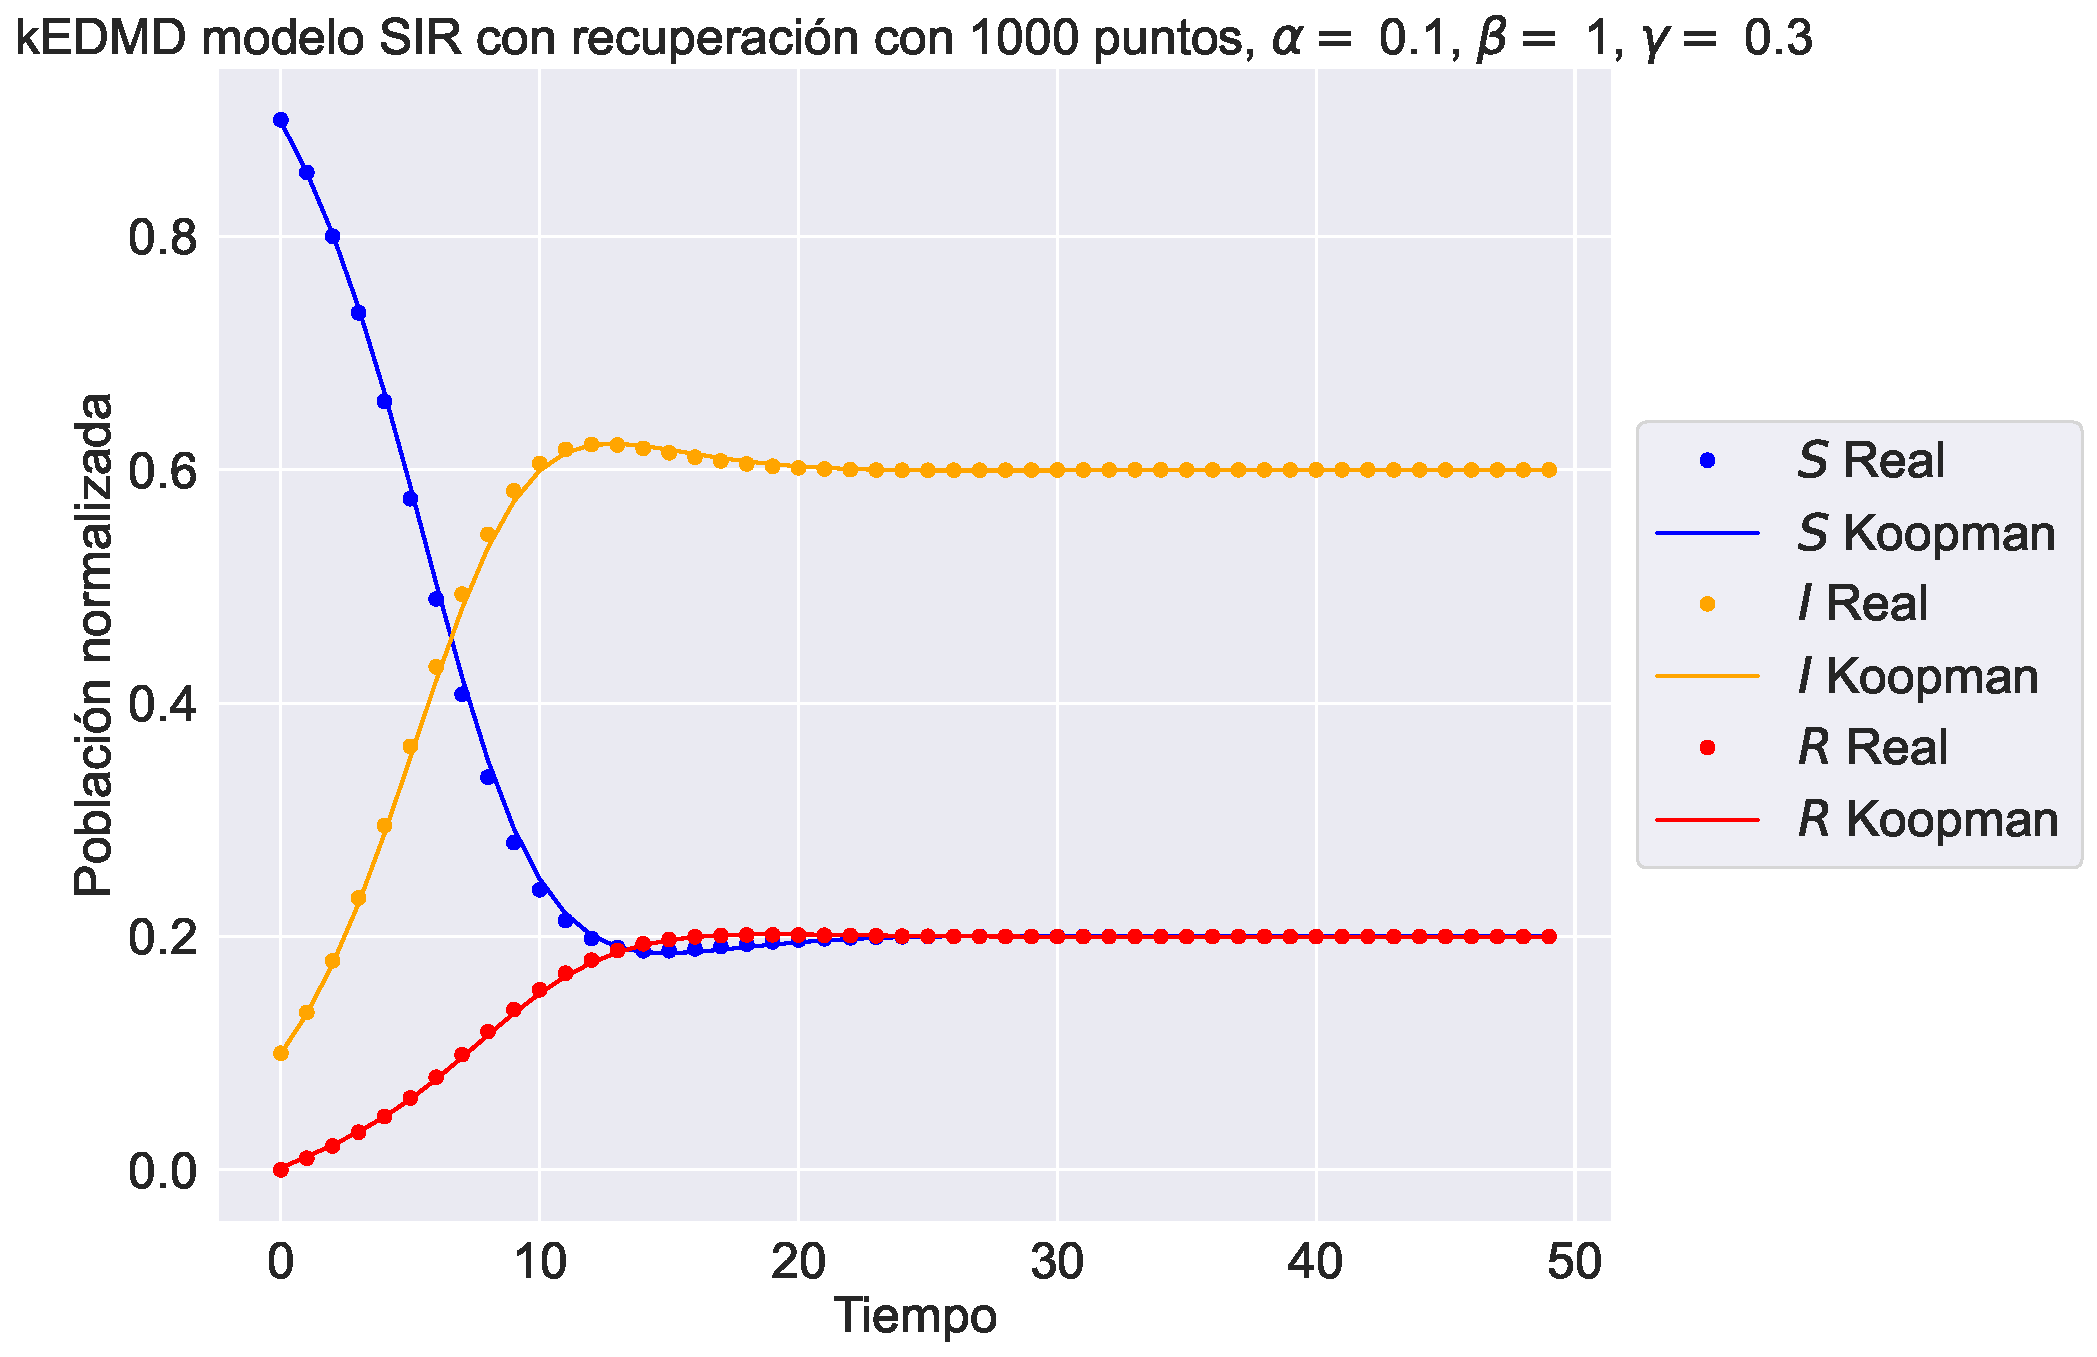
\includegraphics[width=\textwidth]{img/content/chapter3/SIR_rec2.pdf}
        \caption{$\alpha=-0.1$}
        \label{fig:image2}
    \end{subfigure}
    \hfill
    \begin{subfigure}[b]{0.45\textwidth}
        \centering
        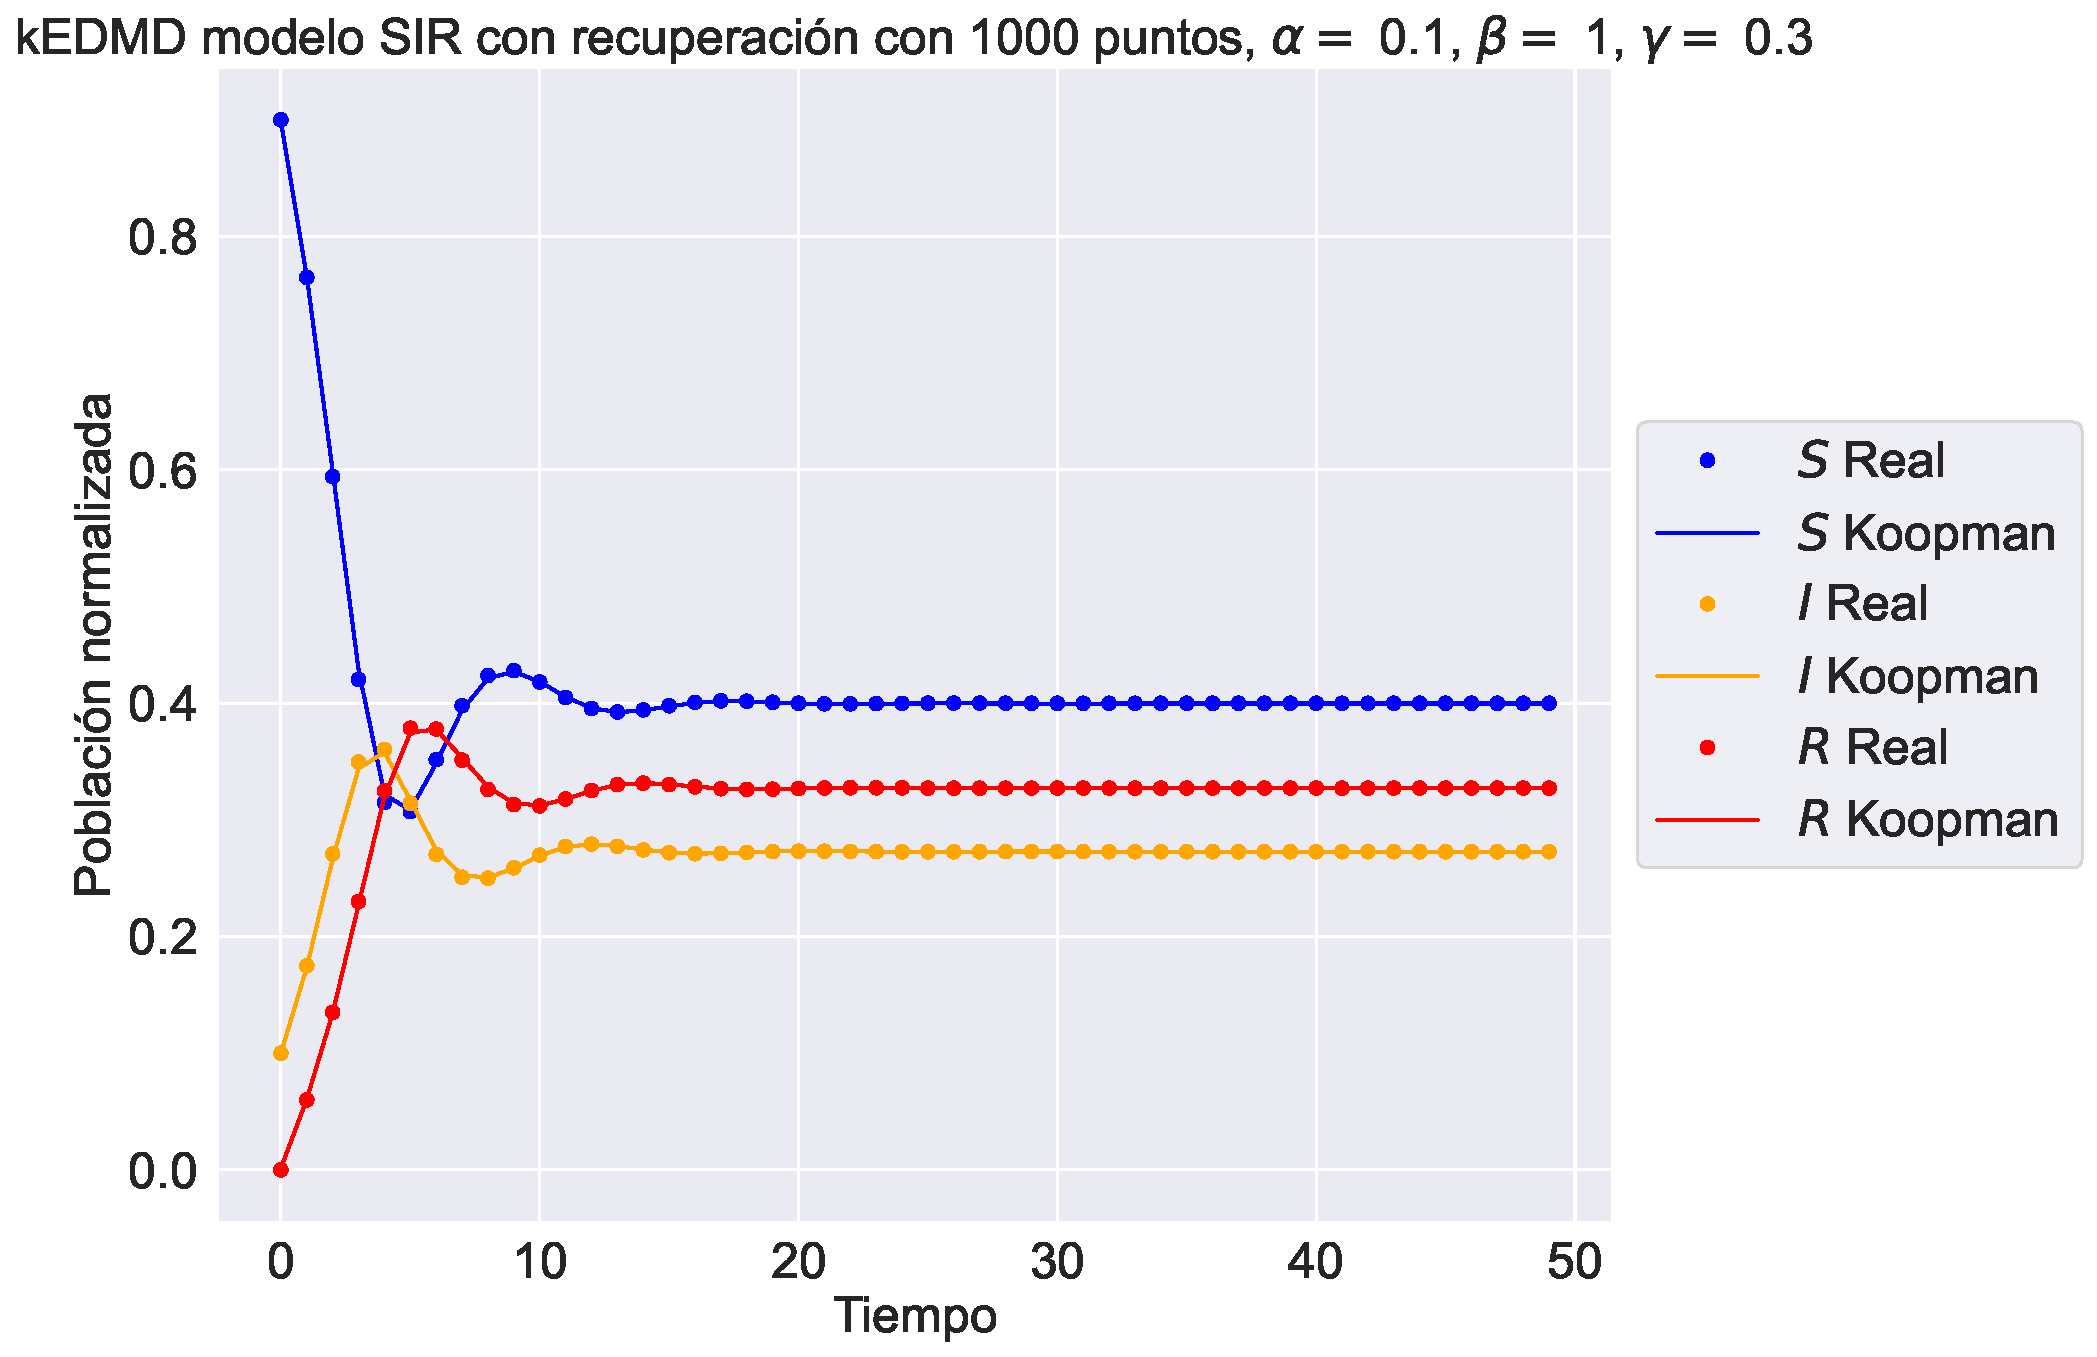
\includegraphics[width=\textwidth]{img/content/chapter3/SIR_rec3.pdf}
        \caption{$\alpha=0.05$}
    \end{subfigure}
    \caption{Ilustración de los tres casos de $\beta$ y $\gamma$ elegidos para la comparación entre el sistema no lineal original y el sistema linealizado por Koopman a 1000 puntos \textit{sampleados} de una variable aleatoria Dirichlet. En forma de puntos se dejan los valores reales que toma el sistema y en línea continua los valores entregados por el sistema linealizado, que se consideran como predicción.}
    \label{fig:Comp_traj_SIR}
\end{figure}
\begin{figure}[h]
    \centering
    \begin{subfigure}[b]{0.32\textwidth}
        \centering
        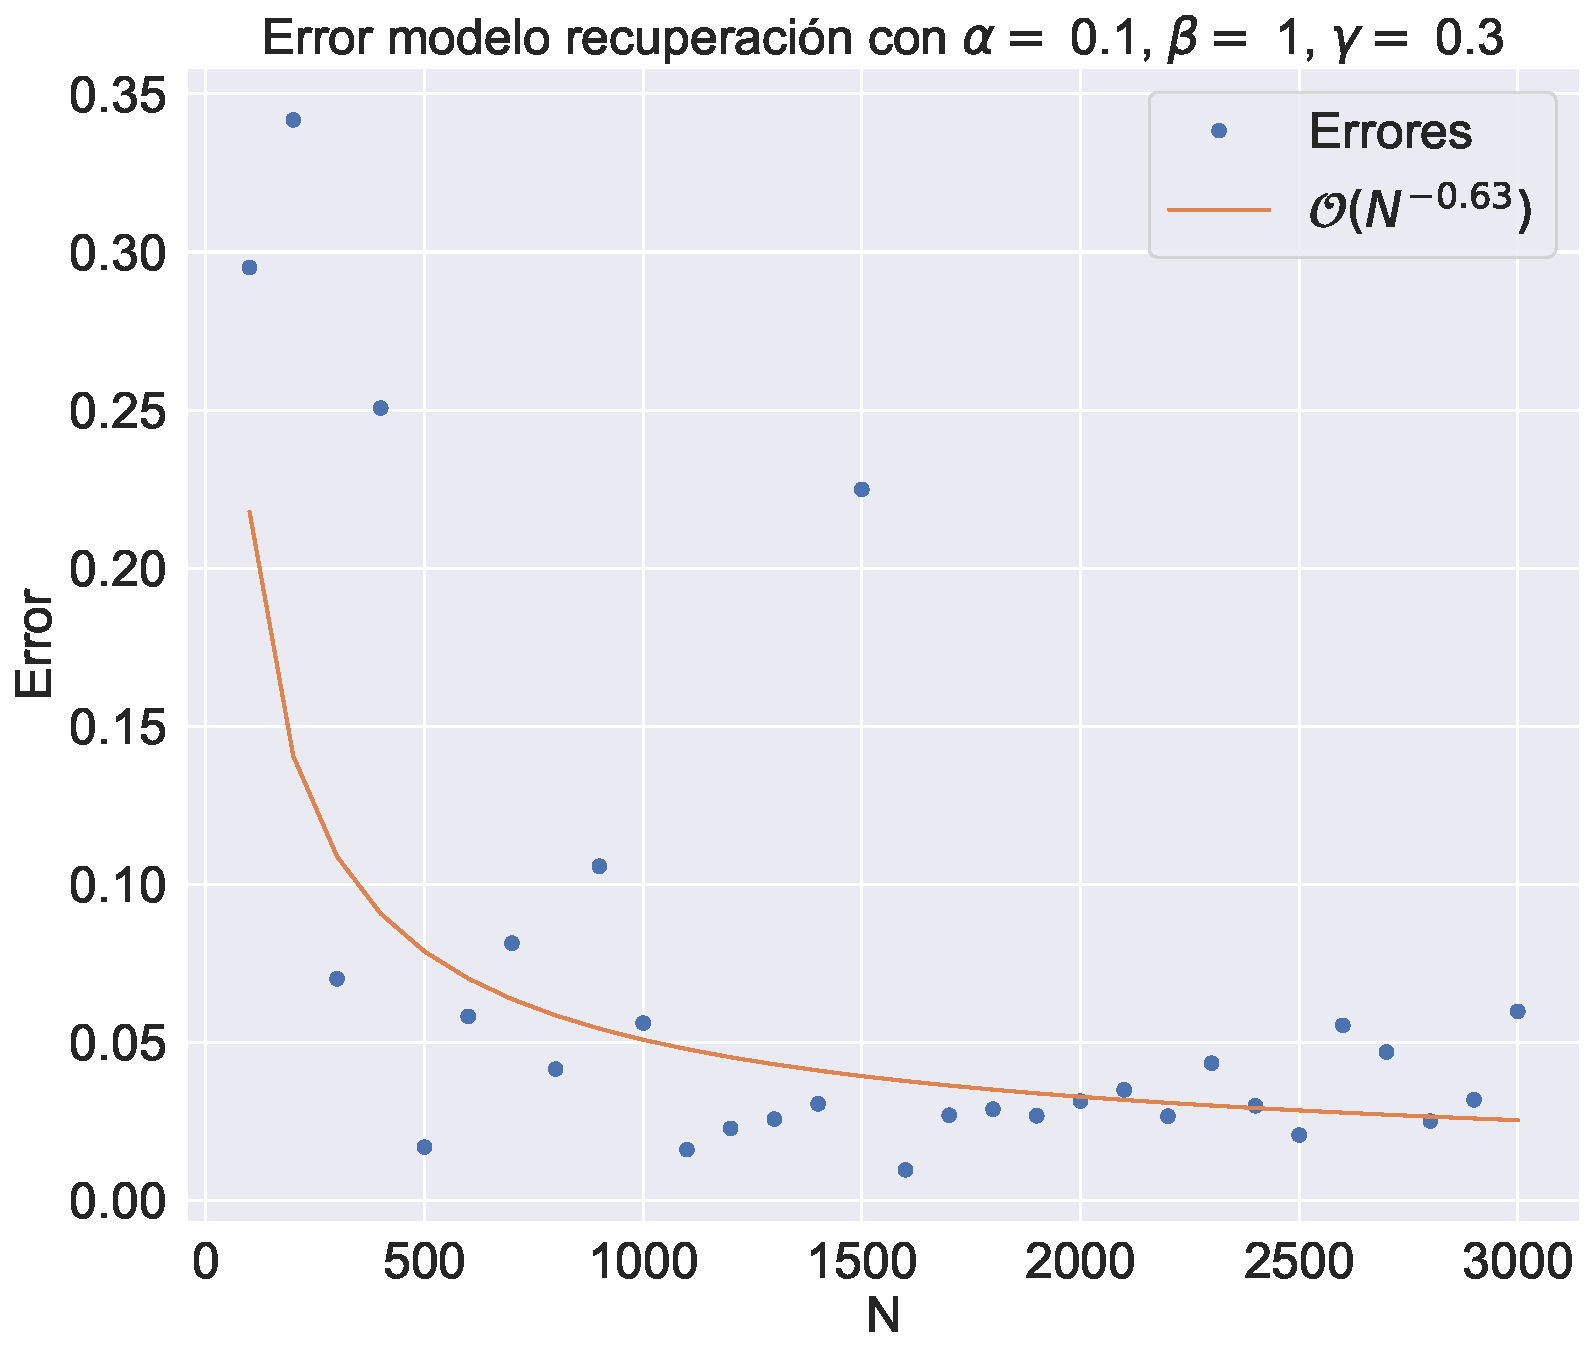
\includegraphics[width=\textwidth]{img/content/chapter3/SIR_rec1Errors.pdf}
        \caption{$\alpha=0.1$, $\beta=1$, $\gamma=0.3$}
    \end{subfigure}
    \hfill
    \begin{subfigure}[b]{0.32\textwidth}
        \centering
        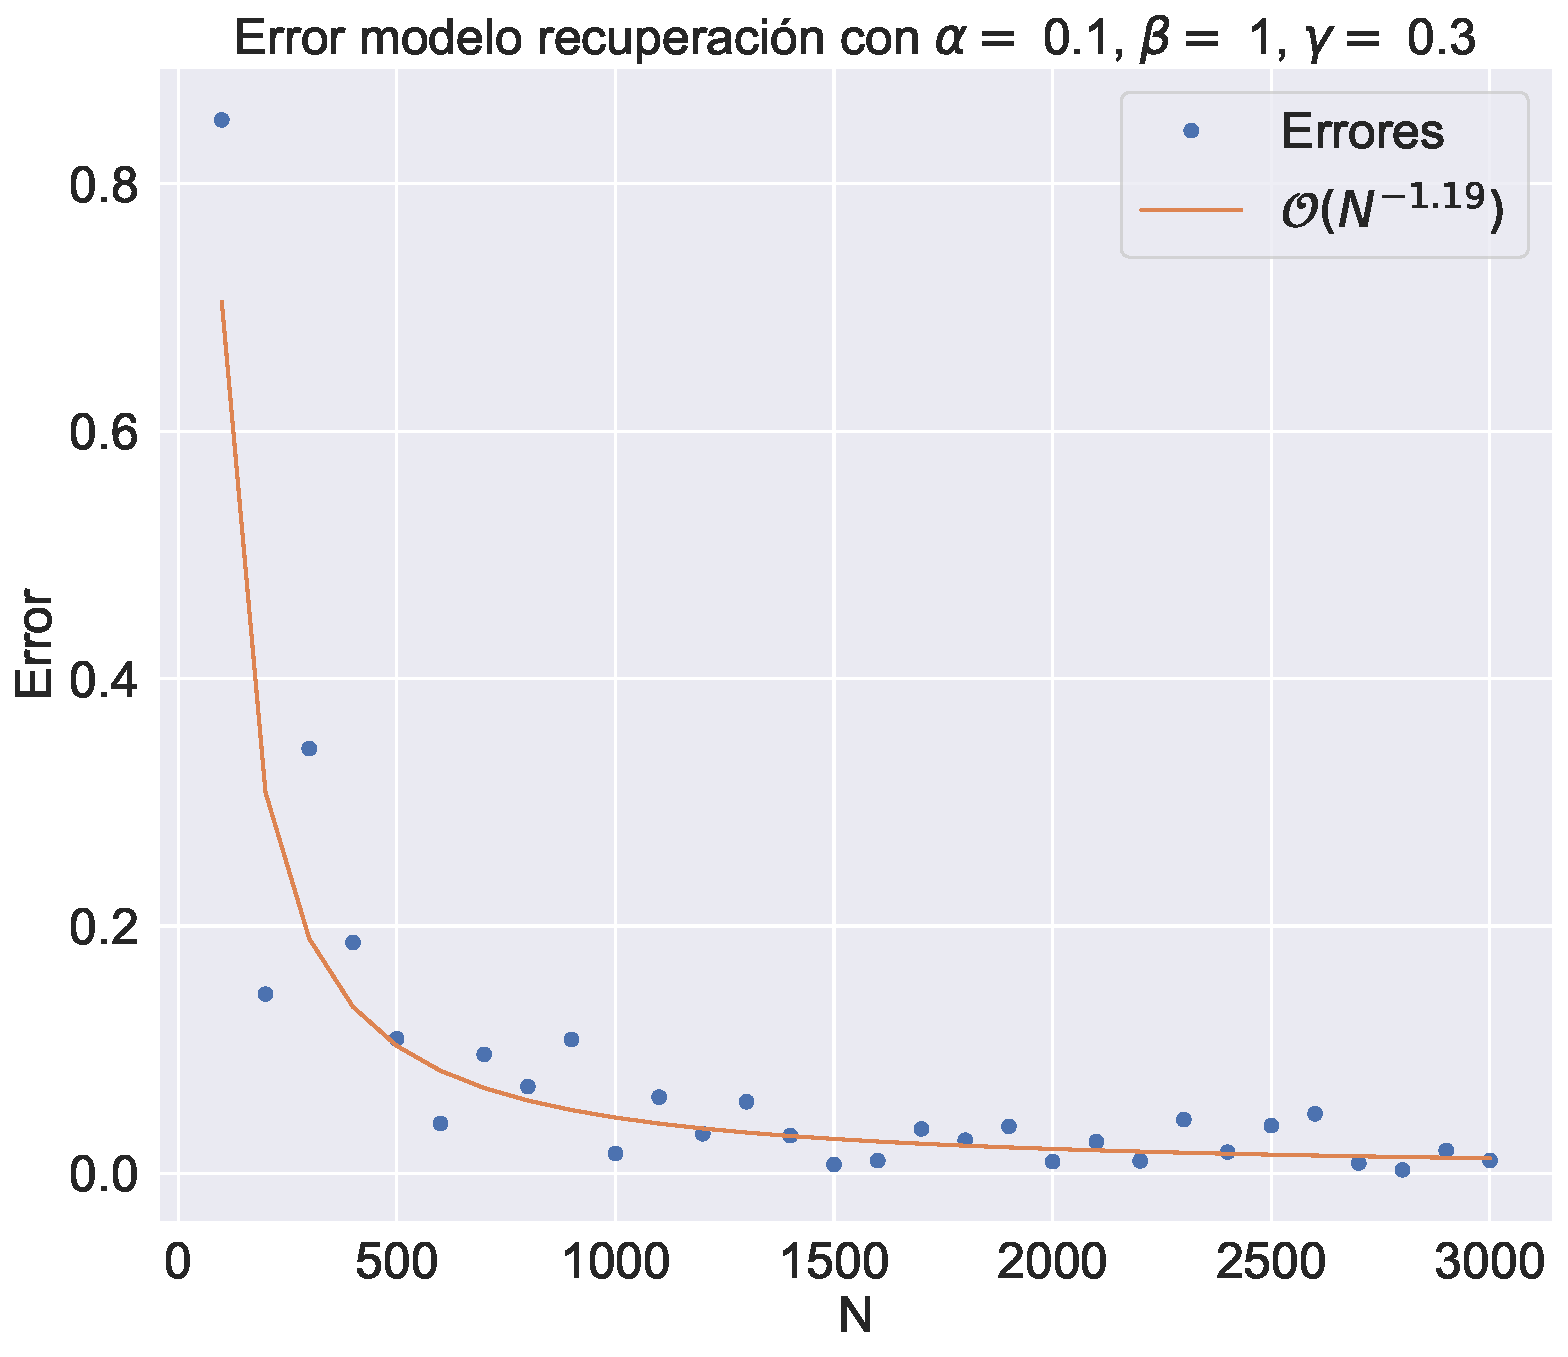
\includegraphics[width=\textwidth]{img/content/chapter3/SIR_rec2Errors.pdf}
        \caption{$\alpha=0.3$, $\beta=1$, $\gamma=0.3$}
    \end{subfigure}
    \hfill
    \begin{subfigure}[b]{0.32\textwidth}
        \centering
        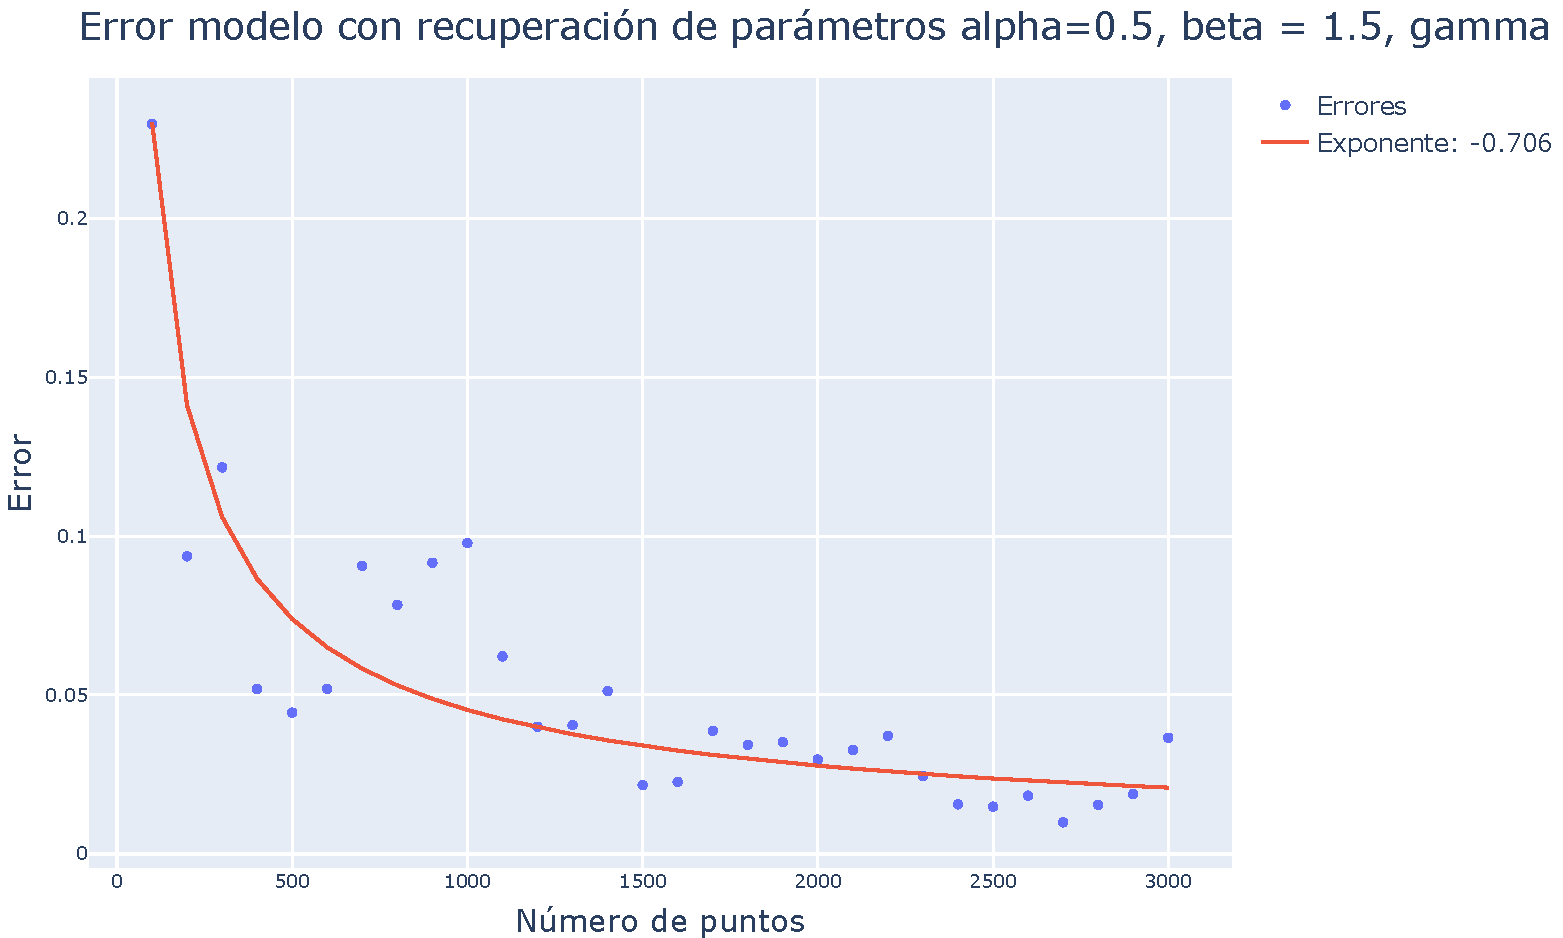
\includegraphics[width=\textwidth]{img/content/chapter3/SIR_rec3Errors.pdf}
        \caption{$\alpha=0.05$}
    \end{subfigure}
    \caption{Ilustración de los tres casos del modelo SIR con pérdida de inmunidad elegido para la evolución en función de $N$ de la diferencia en norma entre el sistema lineal original y el sistema linealizado por Koopman a $N$ puntos,  \textit{sampleados} de una variable aleatoria normal. En forma de puntos se deja la evolución observada del error y en línea continua la mejor curva de la forma $C \cdot N^{a}$, donde $a$ es el exponente que se deja en la leyenda.}
    \label{fig:ErrorSIR_rec}
\end{figure}
Nuevamente se observa que el orden de discrepancia de las trayectorias es de un orden similar, o incluso menor, al visto en la cota \ref{eq:kEDMD_bound}.